\pdfminorversion=4
\makeatletter\let\ifGm@compatii\relax\makeatother
\documentclass[%
    %presentation,
    11pt,
   handout, % Erstellen eines Handouts
]{beamer}
\mode<presentation>
{
  \usetheme{myulm}
  \setbeamercovered{transparent}
}
%\usepackage[ngerman]{babel}
%\usepackage[utf8]{inputenc}
\usepackage[ansinew]{inputenc}
\usepackage{amsmath,amssymb,amsfonts}
\usepackage{times}
\usepackage{graphicx}
\usepackage{fancyvrb}
\usepackage{array}
\usepackage{colortbl}
\usepackage[OT1]{fontenc}
\usepackage{amsthm}
\usepackage{pdfpages}
\usepackage{bbm}
\usepackage{sidecap}
\usepackage[]{subfigure}
\usepackage{graphicx}
\usepackage{enumerate}
\usepackage{rotating}
\usepackage{totpages}
\usepackage[left]{eurosym}
\usepackage{hyperref}
\usepackage{booktabs}
% This is for Anna's symbols
\usepackage{physymb}
\usepackage{tabularx}
\usepackage{multirow}



%\usepackage[breaklinks]{hyperref}

%\usepackage[ansinew]{inputenc}  % ANSI
\usepackage[T1]{fontenc}        % Zeichen-Codierung
\usepackage{textcomp}



%\usepackage{harvard}
\usepackage{natbib}
%\usepackage[longnamesfirst]{natbib}
%\usepackage{har2nat}


%\usepackage{biblatex}
%\bibliography{QCF-literature}


\definecolor{purelightblue}{rgb}{0.93,0.93,1}
\definecolor{pureblue}{rgb}{0.1882,0.2510,0.5647}
\definecolor{UDE}{rgb}{0.1882,0.2510,0.5647}
\setbeamertemplate{blocks}[shadow=true]%[rounded]
\setbeamercolor*{block title}{fg=purelightblue,bg=pureblue}
\setbeamercolor*{block body}{bg=purelightblue}

\definecolor{pcolor}{rgb}{0.0,0.6,0.0}
\definecolor{qcolor}{rgb}{0.75,0.0,0.0}
\definecolor{obscolor}{rgb}{0.58,0.70,0.84}


\newcounter{realpage}


%%%%%%%%%%%%%%%%%%%%%%%%%%%%%%%%%%%%%%%%%%%%%%%%%%%%%%%%%%%%%%%%%%%%%%%%%%%%%%%%%%%%%%%%%


%Anfang der Kopfzeile
\newcommand{\zwischentitel}{}
\newcommand{\leitthema}{Model Risk}
\newcommand{\ort}{Birkbeck College London}


%Anfang zur Titelseite
\title[Pricing II]{MSc Financial Engineering -- Pricing II }
\author{Professor Dr. R{\"u}diger Kiesel}
\newcommand{\presdatum}{Spring 14}
\institute{Birkbeck College}
\subtitle{Lecture Series Spring 2014}
%Ende der Titelseite
\AtBeginPart{
\frame[plain]{\titlepage}
\frame{\partpage}
\frame{\tableofcontents[part=\insertpartnumber]}
}



\AtBeginSection[] % Do nothing for \section*
%{
%\begin{frame}{Agenda}{\quad}
%\only{\tableofcontents[currentsection,hideothersubsections]}
%\end{frame}
%}

\input{../def}
\begin{document}



	

% !TEX root = ModelRisk_spring14UDE.tex

\part{A Theory of Model Risk}

\section{What is Model Risk?}

% frametitle
{SST Classification of Risk Types}
\begin{figure}
	\centering
		\includegraphics[width=0.8\textwidth]{../../../pics/risk_SST}
	\label{fig:Risk_map1}
\end{figure}

% frametitle
{Deutsche Bank Risk Types}
\begin{figure}
	\centering
		\includegraphics[width=0.8\textwidth]{../../../pics/DeutscheBank-RiskTypes}
	\label{fig:Risk_map2}
\end{figure}

% frametitle
{Deutsche Bank Annual Report 2012}
\begin{itemize}
\item<1->
Credit risk, market risk and operational risk attract regulatory capital.
\item<2-> Liquidity risk is the risk arising from our potential inability to meet all payment obligations when they come due or only being able to meet these obligations at excessive costs.
\item<3->Business risk describes the risk we assume due to potential changes in general business conditions, such as our market environment, client behavior and technological progress.
\item<4->Reputational risk is the risk that publicity concerning a transaction, counterparty or business practice involving a client will negatively impact the public's trust in our organization.
\item<5->Furthermore, they mention Insurance specific risk and risk concentration.
\end{itemize}

% frametitle
{Basel Regulation I}
Regulators formulate some principles for models
\begin{itemize}
\item<1-> Uncertainty is specific to the instrument and the point in time the valuation is effected.
\item<2-> A bank is expected to consider all relevant market information likely to have a material effect on an instrument's fair value when selecting the appropriate inputs.
\item<3->Observable inputs or transactions may not be relevant. In such cases, the observable data should be considered, but   may not be determinative.
\end{itemize}

% frametitle
{Basel Regulation II}
\begin{itemize}

\item<1-> There are also operative recommendations
\begin{itemize}
\item Validation includes evaluation of the model's theoretical soundness and mathematical integrity and the appropriateness of model assumptions, including consistency with the market.
\item A bank should use a range of approaches and cross-check validations.
\item Valuation models should be tested and reviewed under possible stress conditions. There should be defined triggers for such reviews.
\end{itemize}

\item<2->
Basel III introduces a risk-invariant leverage ratio of 3 percent in recognition that models may be biased.

\end{itemize}

% frametitle
{Motivation}
\begin{itemize}
\item<1-> Model risk has been recognized as one of the fundamental reasons for financial distress for banks and insurance companies.
Recently, a number of authors addressed this issue:
\begin{itemize}
\item Schoutens et. al. (2004): A perfect calibration - now what?
\item Cont (2006): Model uncertainty and its impact on the pricing of derivative instruments.
\item Bann{\"o}r, Scherer (2011): Quantifying the degree of parameter uncertainty in complex stochastic models
\item Morini, M. (2011): Understanding and Managing Model Risk, Wiley.
\end{itemize}
\item<2-> Important questions:
\begin{itemize}
\item How sensitive is the value of a given derivative to the choice of the pricing model (parametric setting)?
\item Can one quantify a provision for model risk (as for market and credit risk)?
\end{itemize}

\end{itemize}

% frametitle
{Schoutens - CallFit, NIGCIR}
\begin{figure}[htp]
\centering
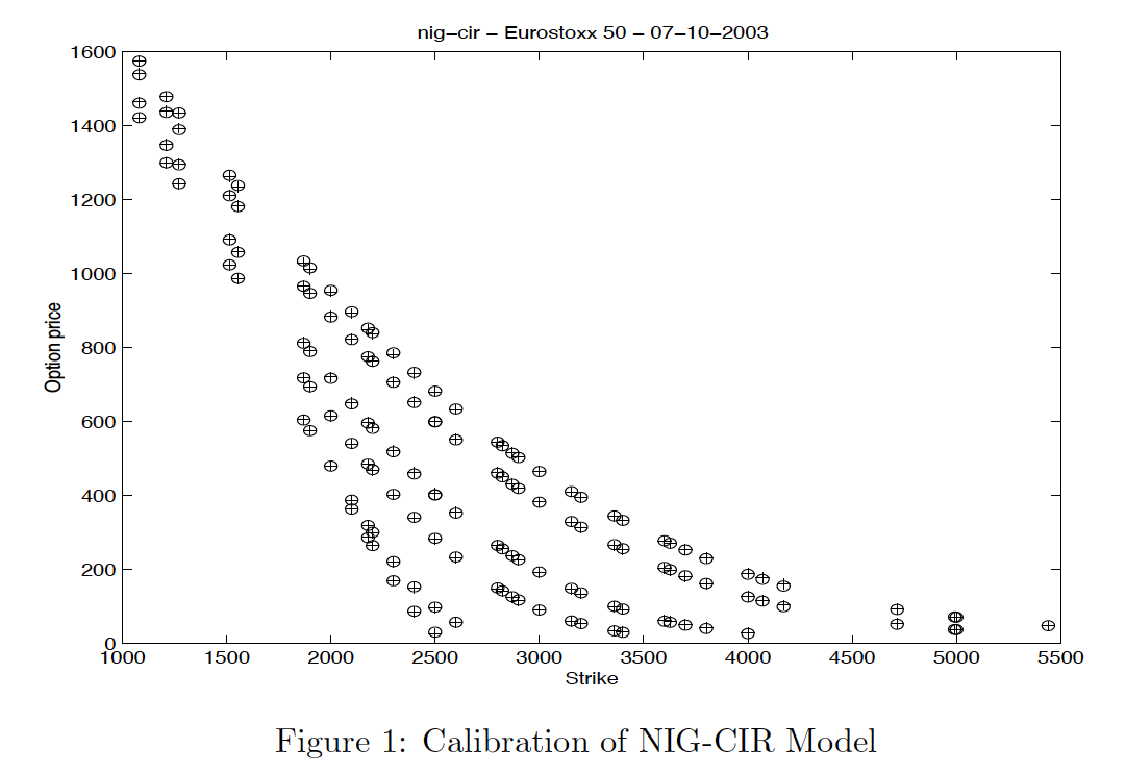
\includegraphics[width=\textwidth]{../../../pics/WS-CallFit.pdf}
\end{figure}

% frametitle
{Schoutens - CallFit, BNS}
\begin{figure}[htp]
\centering
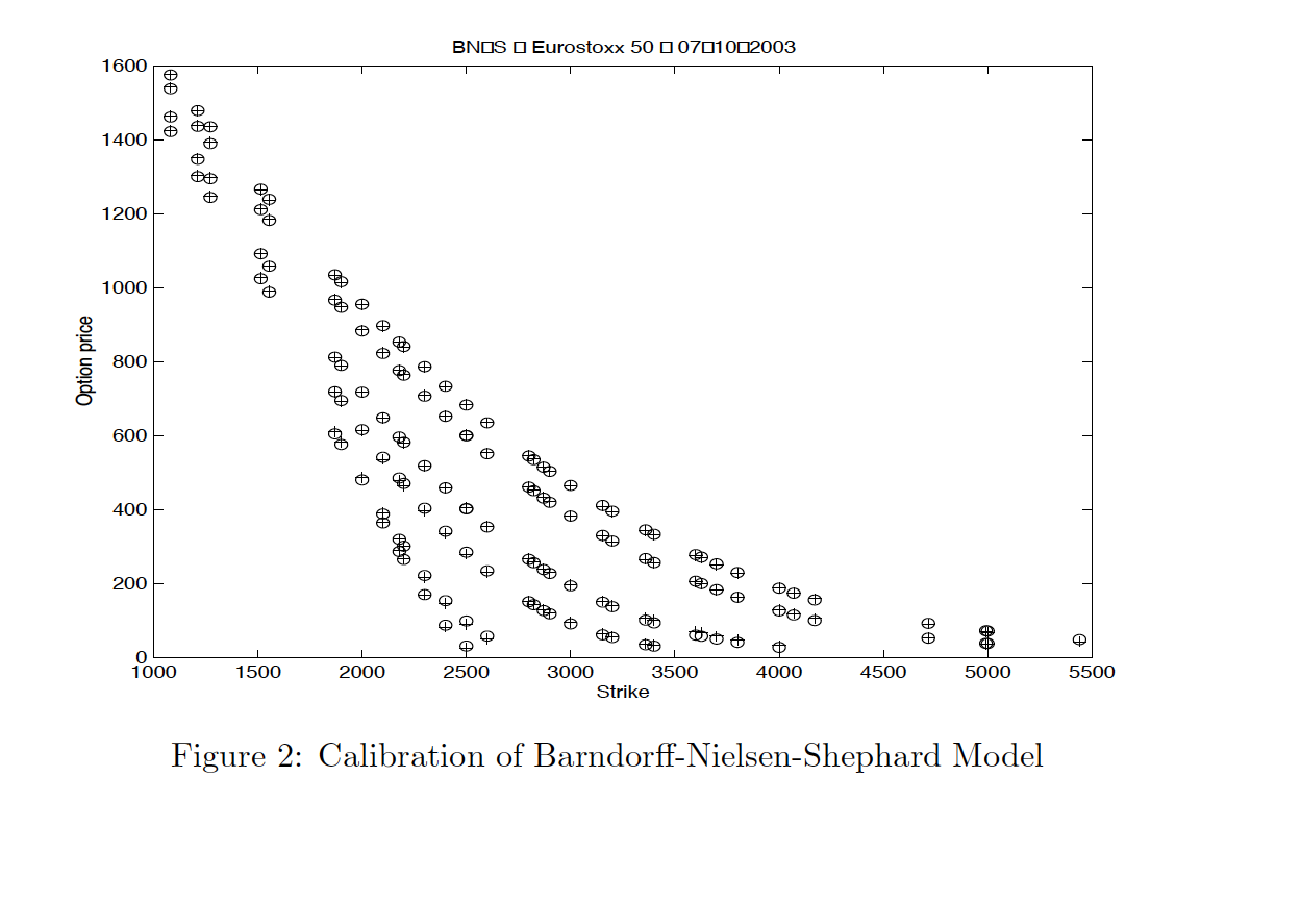
\includegraphics[width=\textwidth]{../../../pics/WS-CallFitBNS.pdf}
\end{figure}

% frametitle
{Schoutens - Exotic Fit}
\begin{figure}[htp]
\centering
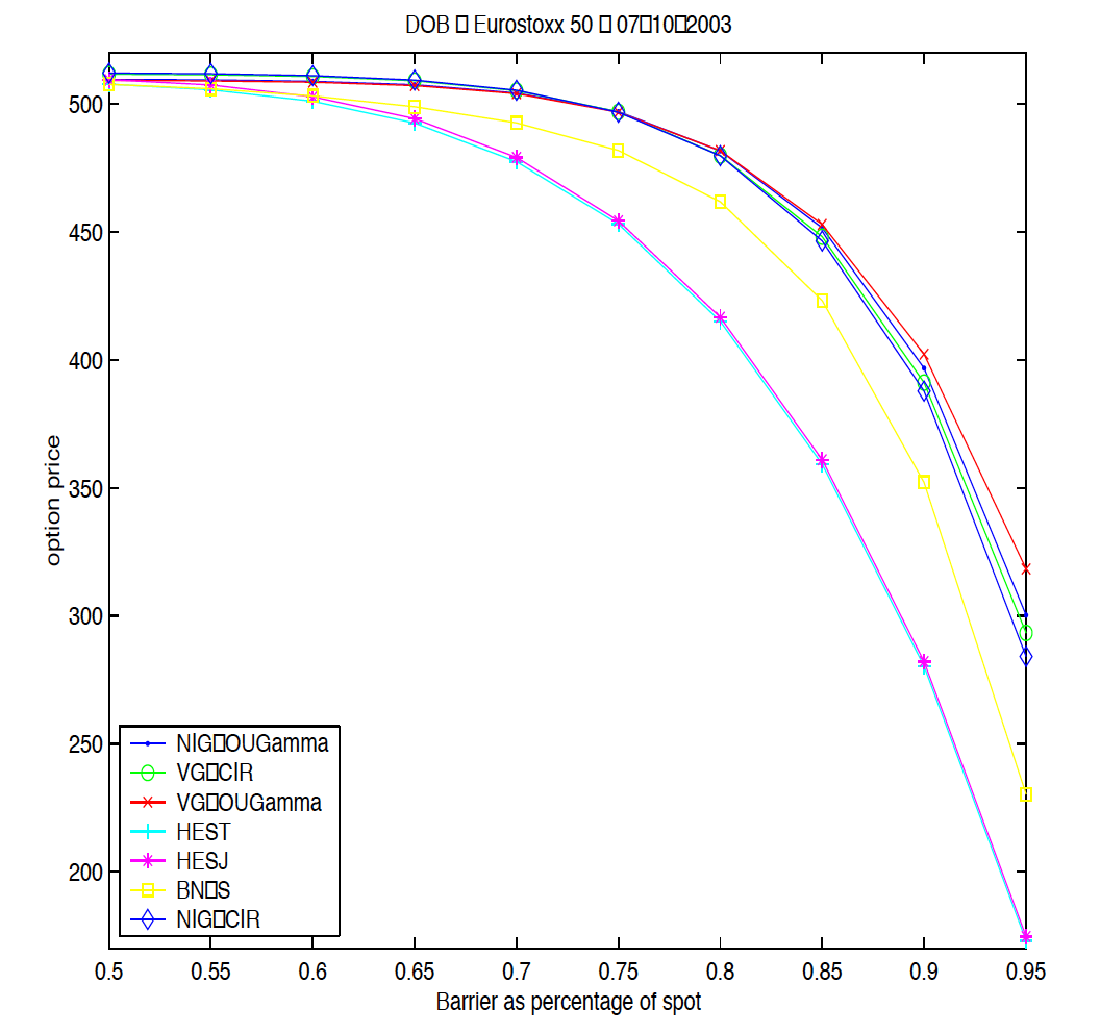
\includegraphics[width=0.7\textwidth, heigth=0.5\textheigth]{../../../pics/WS-ExoticFit.pdf}
\end{figure}

% frametitle
{Schoutens - Clique Fit}
\begin{figure}[htp]
\centering
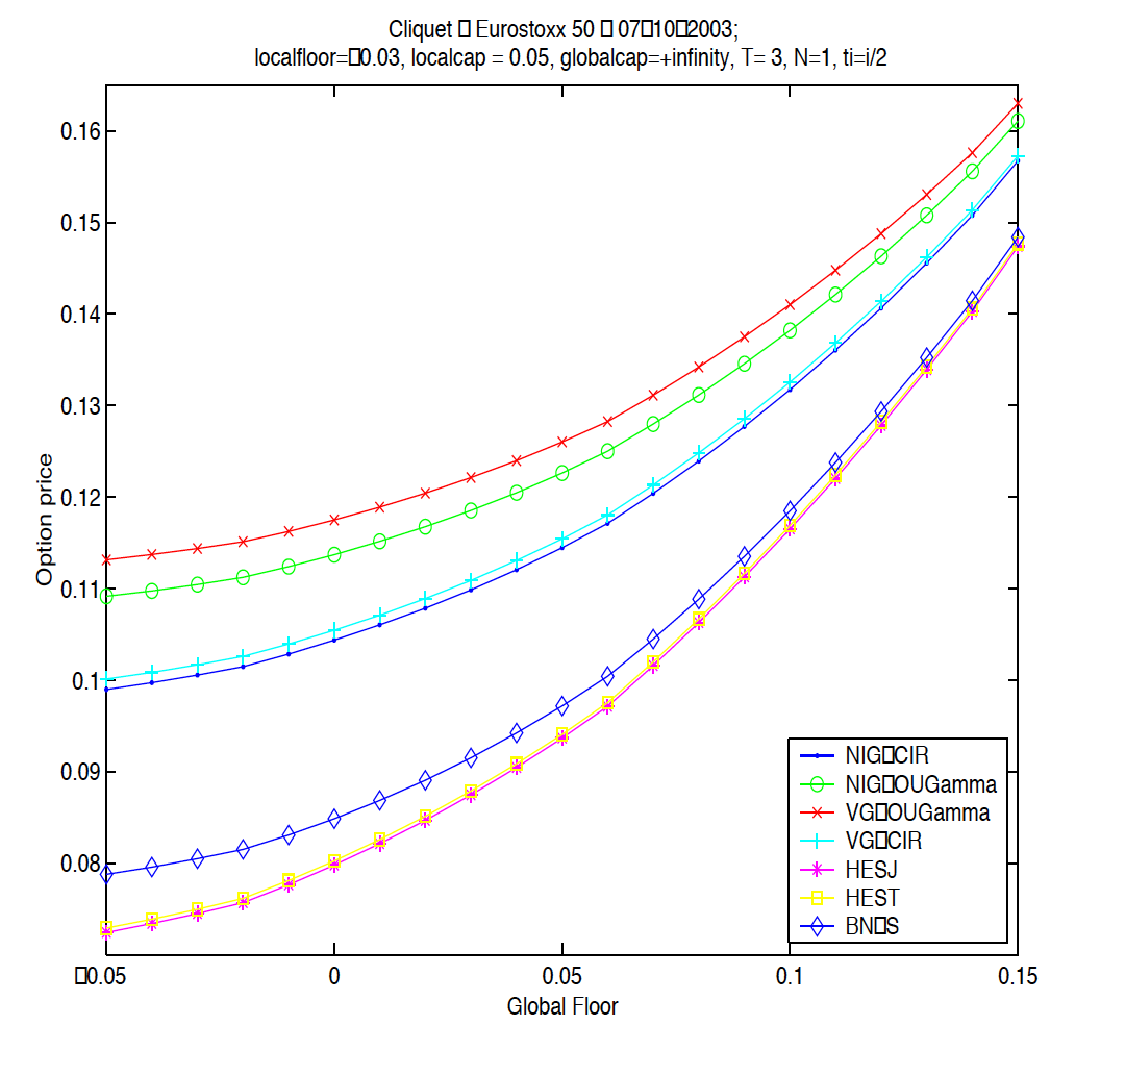
\includegraphics[width=0.7\textwidth, heigth=0.5\textheigth]{../../../pics/WS-CliqueFit.pdf}
\end{figure}

% frametitle
{How to define model risk?}
\begin{itemize}
\item {\it Simple Idea:} Model risk is the possibility that a (financial) institution suffers losses due to mistakes in the development and application of (validation) models.
\end{itemize}

% frametitle
{Derman (1996) -- Value Approach}
\begin{itemize}
\item Is the payoff accurately described?
\item Is the software reliable?
\item Has the model been appropriately calibrated to the prices of the simpler, liquid constituents that comprise the derivative?
\item Does the model provide a realistic description of the factors that affect the derivative's value?
\end{itemize}
Last point: Residual risk relating to the factors -- model risk?

% frametitle
{Rebonato (2003) -- Price Approach}

\begin{itemize}
\item<1-> Model risk is the risk of occurrence of a significant difference between the mark-to-model value of a complex and/or illiquid instrument and the price at which the same instrument is revealed to have traded in the market.
\item<2-> Thus, models can be counterintuitive, unreasonable, maybe not even free of arbitrage, as long as the market agrees with the valuation.
\item<3-> So, large losses  can only happen when a sudden gap opens between market prices and model valuation.
\end{itemize}

% frametitle
{J. Hull: Risk Management and Financial Institutions}
For pricing models are used to
\begin{itemize}
\item<1-> observe model prices for similar instruments that trade
\item<2-> imply model parameters and interpolate as appropriate
\item<3-> value new instrument
\item<4-> perform reverse engineering from prices observed from counterparty quotes to understand their models
\end{itemize}
Model Risk can lead to ..
\begin{itemize}
\item<1->
Incorrect price at time product is bought or sold
\item<2-> Incorrect hedging
\end{itemize}

% frametitle
{Marking Prices of an Instrument to Market}
\begin{itemize}
\item<1->
Use price quoted by market maker (usually financial institutions mark to mid of bid and offer)
\item<2-> Use price at which financial institution has traded product
\item<3-> Use interdealer broker prices
\item<4-> Use interdealer price indications
\item<5-> Use model (marking to model)
\item<6-> Contact member of the trading community
\end{itemize}

% frametitle
{Products}
\begin{itemize}
\item<1-> Linear products: Very little uncertainty about the right model, but mistakes do happen
\item<2-> Standard Products
\begin{itemize}
\item We do not need usually a model to know the price of an actively traded product. The market tells us the price.
\item The model is a communication tool (e.g., implied volatilities are quoted for options)
\item It is also an interpolation tool (e.g., a tool for interpolating between strike prices and maturities)
\end{itemize}
\item<3-> Non-Standard Products
\begin{itemize}
\item In the case of nonstandard products models play a key role in both pricing and hedging
\item It is a good idea to use more that one model whenever possible
\end{itemize}
\end{itemize}

% frametitle
{Hull: Model Risk}
\begin{itemize}
\item<1->  Dangers in Model Building
\begin{itemize}
\item Overfitting
\item Overparametrization
\end{itemize}
\item<2-> Detecting Model Problems
\begin{itemize}
\item<1-> Monitor types of trading a financial institution is doing with other financial institutions
\item<2-> Monitor profits being recorded from trading of different products (over- reap. under-pricing).
\item<3-> Use Model Audit Group
\begin{itemize}
\item Check that a model has been implemented correctly
\item Examine whether there is a sound rationale for the model
\item Compare the model with others that can accomplish the same task
\item Specify limitations of model
\item Assess uncertainties in prices and hedge parameters given by model
\end{itemize}
\end{itemize}
\end{itemize}

\section{Tools to Assess Model Risk}
\subsection{Risk, Uncertainty, and Ambiguity}

% frametitle
{Definitions}
\begin{itemize}
\item<1-> Typically a stochastic model $(\Omega, \F)$ defining future scenarios and a
probability measure $\prob$ on these outcomes.
\item<2->  We have to distinguish between
\begin{itemize}
\item {\it Risk:}  we are able to specify a unique $\prob$
\item {\it (Knightian) Uncertainty:} we are not able to specify a precise $\prob$
\item {\it Ambiguity:}  we are facing several possible specifications $\prob_1, \prob_2, \ldots$\end{itemize}
\item<3-> Approaches to deal with ambiguity are "averaging" and "worst-case".
\end{itemize}

% frametitle
{Bayesian Model Averaging}
\begin{itemize}
\item<1-> Let ${\cal M}= \{M_1, \dots, M_J\}$ be a family of models and  $\{\Theta_1, \dots, \Theta_J\}$ the corresponding parameter spaces.
\item<2->  A Bayesian observer has
\begin{itemize}
\item a prior on model parameters $p(\theta_j|M_j)$
\item a prior on model weights $\prob(M_j)$
\end{itemize}
\item<3-> Given a set of observations $y$ the posterior probabilities are
$$
\prob(M_j|y) = \frac{p(y|M_j)\prob(M_j)}{\sum_{k=1}^{J}p(y|M_k)\prob(M_k)}
$$
with
$$
p(y|M_j)=\int_{\Theta_j} \prob(y|\theta_j, M_j)p(\theta_j|M_j) d\theta_j.
$$
\end{itemize}

% frametitle
{Bayesian Model Averaging -- Valuation}
\begin{itemize}
\item<1-> If we want to compute a model dependent quantity $X$ given by an expectation we average over models.
\item<2-> Given a set of observations $y$ the posterior expectation is
$$
\EX(X|y) = \sum_{j=1}^{J} \EX(X |y, M_j) \prob(M_j |y).
$$
\item<3-> Problems:
\begin{itemize}
\item how to specify priors (stock vol vs jump diffusion?)
\item computational intensive
\end{itemize}

\end{itemize}

% frametitle
{Worst-Case Approach}
\begin{itemize}
\item<1-> The worst-case approach has its foundations in the "MaxMin" approach as a robust version of expected utility. \item<2-> Assume $U$ is a utility function, then
$$
\max _X \min_{\prob \in {\cal P}} \EX_{\prob}(U(X)).
$$
\item<3-> Separation of risk-aversion and aversion to ambiguity
\begin{itemize}
\item risk aversion is captured in $U$
\item aversion to ambiguity is captured in $\min$
\end{itemize}

\end{itemize}

\subsection{Risk Measures}

% frametitle
{Convex Risk Measures}

Let $(\Omega, \F)$ be a measurable space and ${\cal X} \subset {\cal L}^0(\Omega)$ a vector space. ${\cal Y} \subset {\cal X}$ be a sub-vector space and
$\pi \in {\cal Y}^*$.
\begin{equation}
\rho: {\cal X} \rightarrow \setR
\end{equation}
is a convex risk measure with $\pi$ translation invariance iff
\begin{itemize}
\item $\rho$ is monotone: $$X \leq Y \;  \implies \; \rho(X) \geq \rho(Y).$$
\item $\rho$ is convex: $$\forall \lambda \in [0,1]: \rho(\lambda X + (1-\lambda) Y) \leq \lambda \rho(X) + (1-\lambda) \rho(Y).$$
\item $\rho$ is $\pi$-translation invariant: $$\forall Y \in {\cal Y}: \rho(X+Y) = \rho(X) + \pi(Y).$$
\end{itemize}

% frametitle
{Coherent Risk Measures}

A coherent risk measure is a function $\rho$ on abstract risk positions such that
\begin{itemize}
\item<1-> \emph{Monotonicity}: if $X\geq 0$, then $\rho(X)\leq 0$;
\item<2-> \emph{Translation invariance}: if $k \in \R$, then
$\rho(X+k)=\rho(X)-k$;
\item<3-> \emph{Homogeneity}: if $\lambda \geq 0$ in $\R$, then $\rho(\lambda X)
= \lambda \rho (X)$;
\item<4-> \emph{Subadditivity}: $\rho(X+Y)\leq \rho(X)+\rho(Y)$.
\end{itemize}

% frametitle
{Convex Risk Measures -- Properties}

\begin{itemize}
\item $\rho$ is coherent $\Leftrightarrow \; \rho(cX) = c \rho(X), \; \forall c>0$.
\item $\rho$ is normalized $\Leftrightarrow \; \rho(0) = 0$.
\item Let $\prb$ be a probability measure on $(\Omega, \F)$.\\
$\rho$ is $\prb$-law invariant $\Leftrightarrow \; \prb^X = \prb^Y $ implies $\rho(X) = \rho(Y)$.
\end{itemize}

% frametitle
{Examples: VaR and AVaR}
\begin{itemize}
\item general probability space $(\Omega, \F, \prb)$, $\beta \in (0,1]$, $X\in L^1(\prb)$, then
$$
VaR_\beta(X) = q_{-X}^{\prb}(1-\beta).
$$
 \item VaR is not a coherent risk measure as it is not subadditive in general.
\item the average value at risk at level $\alpha \in (0,1]$ is
$$
AVaR_\alpha(X) = \frac{1}{\alpha} \int_0^\alpha VaR_\beta(X) d\beta.
$$
\item AVaR$_\alpha$ is a convex risk measure (coherent and law-invariant).
\end{itemize}

% frametitle
{Value at Risk}
The worst $1-\alpha$ scenarios are below the $-VaR_\alpha$, all others are below.
\begin{figure}
	\centering
		\includegraphics[width=0.8\textwidth]{../../../pics/VaR}
	\label{fig:VaR}
\end{figure}

% frametitle
{Value at Risk}
The figure illustrates a portfolio with a low VaR compared to its risk.
\begin{figure}
	\centering
		\includegraphics[width=0.7\textwidth]{../../../pics/Shortcoming_VaR}
	\label{fig:Shortcoming_VaR}
\end{figure}

% frametitle
{Average Value-at-Risk (AVaR) }
\begin{itemize}
\item<1-> The AVaR specifies the expectation of the loss in case the loss is above the VaR.
\item<2-> AVaR is also called Tail Value-at-Risk (TVaR) or Conditional
Value-at-Risk (CVaR) or  Expected Shortfall (ES).
\end{itemize}

% frametitle
{Illustration of AVaR}
\begin{figure}
	\centering
		\includegraphics[width=1\textwidth]{../../../pics/Expected_Shortfall}
	\label{fig:Expected_Shortfall}
\end{figure}

\section{Stochastic Models of Financial Markets}
\subsection{Model Setting}

% frametitle
{ Financial Market Model}
\begin{itemize}
\item<1->
$T>0$ is a fixed a planning horizon.
\item<2->
Uncertainty in the financial market is modelled by a probability
space $(\Omega, {\cal F},\prb)$ and an information set  (filtration) $\fil =({\cal
F}_t)_{0\leq t\leq T}$.
\item<3->
There are $d+1$ primary traded assets, whose price processes are
given by stochastic processes $S_0, \ldots, S_d$, which represent
the prices of some traded assets.
\item<4->
A num\'{e}raire is a price process $X(t)$ almost surely strictly
positive for each $t \in [0,T]$.
\item<5->
\lq {Historically}' the money market account $B(t)=e^{rt}$ with a
positive constant $r$ was used as a
num\'{e}raire.
\end{itemize}

% frametitle
{ Trading Strategies}

\begin{itemize}
\item<1->  We call an $\setR^{d+1}$-valued process
$$
\varphi(t) = (\varphi_0(t), \ldots, \varphi_d(t)), \A t \in [0,T]
$$
a trading strategy (or dynamic portfolio process).
\item<2->
Here $\varphi_i(t)$ denotes the number of shares of asset $i$ held
in the portfolio at time $t$ - to be determined on the basis of
information available {\it before} time $t$; i.e. the investor
selects his time $t$ portfolio after observing the prices $S(t-)$.
\end{itemize}

% frametitle
{ Trading Strategies}
\begin{itemize}
\item<1->  The value of the portfolio $\varphi$ at time $t$ is
given by
$$
V_\varphi(t) :=  \varphi(t) \cdot S(t) = \sum_{i=0}^d \varphi_i(t)
S_i(t).
$$
$V_\varphi(t)$ is called the value process, or wealth process, of
the trading strategy $\varphi$.\ \item<2-> The gains process
$G_\varphi(t)$ is
$$
G_\varphi(t) := \sum_{i=0}^d \int_0^t \varphi_i(u) dS_i(u).
$$
\item<3-> A trading strategy $\varphi$ is called self-financing if
the wealth process $V_\varphi(t)$ satisfies
$$
V_\varphi(t) = V_\varphi(0) + G_\varphi(t)\A \mbox{for all}\; t\in
[0,T].
$$
\end{itemize}

% frametitle
{ Discounted Processes}

The discounted price process is
$$
\td{S}(t) := \frac{S(t)}{S_0(t)} = (1, \td{S}_1(t), \ldots
\td{S}_d(t))
$$
with $\td{S}_i(t) = S_i(t)/S_0(t),\; i=1,2, \ldots, d$. The
discounted wealth process $\td{V}_\varphi(t)$ is
$$
\td{V}_\varphi(t):= \frac{V_\varphi(t)}{S_0(t)} = \varphi_0(t) +
\sum_{i=1}^d \varphi_i(t) \td{S}_i(t)
$$
and the discounted gains process $\td{G}_\varphi(t)$ is
$$
\td{G}_\varphi(t) := \sum_{i=1}^d \int_0^t \varphi_i(t)
d\td{S}_i(t).
$$

% frametitle
{ Self-Financing}

$\varphi$ is self-financing if and only if
$$
\td{V}_\varphi(t) = \td{V}_\varphi(0) + \td{G}_\varphi(t).
$$

Thus a self-financing strategy is completely determined by its
initial value and the components $\varphi_1, \ldots, \varphi_d$.
Any set of processes $\varphi_1, \ldots, \varphi_d$
such that the stochastic integrals $\int \varphi_i d\td{S}_i$
exist can be uniquely extended to a self-financing strategy
$\varphi$ with specified initial value $\td{V}_\varphi(0)= v$ by
setting the cash holding as
$$
\varphi_0(t) = v + \sum_{i=1}^d \int_0^t \varphi_i(u) d\td{S}_i(u)
- \sum_{i=1}^d \varphi_i(t) \td{S}_i.
$$

\subsection{Arbitrage and Equivalent Martingale Measures}

% frametitle
{ Arbitrage Opportunities}

A self-financing trading strategy $\varphi$ is called an arbitrage
opportunity if the wealth process $V_\varphi$ satisfies the
following set of conditions:
$$
V_\varphi(0)=0,\A \prb(V_\varphi(T) \geq 0) =1,
$$
and
$$
\prb(V_\varphi(T) > 0) >0.
$$

%\subsection{Equivalent Martingale Measures}

% frametitle
{ Martingale Measure}

A probability measure $\Q$ defined on $(\Om,\F)$ is an equivalent
martingale measure (EMM) if:\\*[6pt]
(i) $\Q$ is equivalent to $\prb$,\\
(ii) the discounted price process $\td{S}$ is a $\Q$ martingale.

Assume $S_0(t) = B(t) = e^{rt}$, then $\Q \sim \prb$ is a
martingale measure if and only if every asset price process $S_i$
has price dynamics under $\Q$ of the form
$$
dS_i(t) = r S_i(t) dt + dM_i(t),
$$
where $M_i$ is a $\Q$-martingale.

% frametitle
{ EMMs and Arbitrage}

Assume $\Q$ is an EMM. Then the market model contains no arbitrage
opportunities.

{\it Proof.} Under $\Q$ we have that $\td{V}_\varphi(t)$ is a
martingale. That is,
$$
\EX_{\Q}\left(\td{V}_\varphi(t)|\F_u\right) = \td{V}_\varphi(u),\;
\mbox{ for all }\A u \leq t \leq T.
$$
For $\varphi \in \Phi$ to be an arbitrage opportunity we must have
$\td{V}_\varphi(0) =V_\varphi(0)= 0$.  Now
$$
\EX_{\Q}\left(\td{V}_\varphi(t)\right) = 0,\; \mbox{ for all } 0
\leq t \leq T.
$$

% frametitle
{ EMMs and Arbitrage}

Now $\td{V}_\varphi(t)$ is a martingale, so
$$
\EX_{\Q}\left(\td{V}_\varphi(t)\right) = 0,\; 0 \leq t \leq T,
$$
in particular $ \EX_{\Q}\left(\td{V}_\varphi(T)\right) = 0. $

For an arbitrage opportunity $\varphi$ we have $
\prb\left(V_\varphi(T) \geq 0\right) =1, $ and since $\Q \sim
\prb$, this means $ \Q\left(V_\varphi(T) \geq 0\right) =1. $

Both together yield
$$
\Q\left(V_\varphi(T) > 0\right) = \prb\left(V_\varphi(T) >
0\right) =0,
$$
and hence the result follows.\hfill \eb

% frametitle
{ Contingent Claims}

A contingent claims $X$ is a random variable with existing expected value.
\begin{itemize}
\item<1-> A contingent claim $X$ is called attainable if there
exists at least one admissible trading strategy such that
$$
V_\varphi(T) = X.
$$
We call such a  trading strategy $\varphi$ a replicating strategy
for $X$. \item<2-> The financial market model ${\cal M}$ is said
to be complete if any contingent claim is attainable.

\end{itemize}

% frametitle
{ No-Arbitrage Price}

If a contingent claim $X$ is attainable, $X$ can be replicated by
a portfolio $\varphi \in \Phi(\prb^*)$. This means that holding
the portfolio and holding the contingent claim are equivalent from
a financial point of view. In the absence of arbitrage the
(arbitrage) price process $\Pi_X(t)$ of the contingent claim must
therefore satisfy
$$
\Pi_X(t) = V_\varphi(t).
$$

% frametitle
{ Risk-Neutral Valuation}

The arbitrage price process of
any attainable claim is given by the risk-neutral valuation
formula
$$
\Pi_X(t) = S_0(t)
\EX_{\prb^*}\left[\left.\frac{X}{S_0(T)}\right|\F_t\right].
$$

Thus, for any two replicating portfolios $\varphi, \psi \in
\Phi(\prb^*)$
$$
V_\varphi(t) = V_\psi(t).
$$

% frametitle
{ Risk-Neutral Valuation}

{\it Proof.} Since $X$ is
attainable, there exists a replicating strategy $\varphi \in
\Phi(\prb^*)$ such that $V_\varphi(T) = X$ and $\Pi_X(t) =
V_\varphi(t)$. Since $\varphi \in \Phi(\prb^*)$ the discounted
value process $\td{V}_\varphi(t)$ is a martingale, and hence
$$
\begin{array}{lll}
\Pi_X(t) &=&\DSE V_\varphi(t) = S_0(t)\td{V}_\varphi(t) \\*[12pt]
&=&\DSE S_0(t) \EX_{\prb^*}
\left[\left.\td{V}_\varphi(T)\right|\F_t\right]\\*[18pt]
&=&\DSE S_0(t)
\EX_{\prb^*}
\left[\left.\frac{V_\varphi(T)}{S_0(T)}\right|\F_t\right]\\*[18pt]
&=&\DSE S_0(t) \EX_{\prb^*}
\left[\left.\frac{X}{S_0(T)}\right|\F_t\right]\!.
\end{array}
$$
\hfill \eb

\subsection{Black-Scholes Model}

% frametitle
{ Black-Scholes Model}

The classical Black-Scholes model is
$$
\begin{array}{llll}
dB(t) &=&\DSE r B(t) dt, \A &B(0)= 1,\\ dS(t) &=&\DSE S(t) \left(
b dt + \sigma dW(t) \right)\!, \A &S(0) = p,
\end{array}
$$
with constant coefficients $b \in \setR,\; r,\s \in \setR_+$.

The Black-Scholes price pro\-cess of a European call is given by
$$
\begin{array}{lll}
C(t) &=&\DSE S(t) \Phi(d_1(S(t), T-t))\\*[12pt] &&- K e^{-r(T-t)}
\Phi(d_2(S(t), T-t)).
\end{array}
$$
The functions $d_1(s,t)$ and $d_2(s,t)$ are given by
$$
\begin{array}{lll}
d_1(s,t) &=&\DSE \frac{\log(s/K) + (r +
\frac{\sigma^2}{2})t}{\sigma \sqrt{t}},\\*[12pt] d_2(s,t) &=&\DSE
 \frac{\log(s/K) + (r -
\frac{\sigma^2}{2})t}{\sigma \sqrt{t}}
\end{array}
$$

\section{Quantitative Frameworks for Model Risk}
\subsection{Parametric Model Risk}

% frametitle
{Parameter uncertainty}
\begin{itemize}
\item $(\Omega, \F, \fil)$ filtered measurable space
\item $S= (S_t)$ basic instruments, contingent claim $X=F(S)$
%\item contingent claims discounted with matching numer{\'a}ire
\item parametrized family of (martingale) measures $(\Q_\theta)_{\theta \in \Theta}$ on $(\Omega, \F)$.
\item parameter $\theta \in \Theta$, (risk neutral) value of contingent claim is
$$
\theta \rightarrow \EX_\theta(X) := \EX_{\Q_\theta}(X).
$$

\end{itemize}

% frametitle
{Parameter Uncertainty}
To use models we need to specify the parameters
\begin{itemize}
\item<1-> estimation
\begin{itemize}
\item some estimator $\hat{\vartheta}$ is used instead the true parameter $\vartheta$
\item bias and volatility of the estimator have to be considered
\end{itemize}
\item<2-> calibration
\begin{itemize}
\item search for parameter that minimizes some pricing error condition, e.g.
$$
\vartheta_c = \argmin_{\vartheta} \left| \sum_{\mbox{\tiny set of derivatives}} \mbox{model price} (\vartheta) - \mbox{market price} \right|
$$
\item parameters may not be uniquely identified
\end{itemize}
\item<3-> Both approaches
\begin{itemize}
\item produce parameter uncertainty,
\item may disregard information.
\end{itemize}
\end{itemize}

% frametitle
{Bann{\"o}r-Scherer Approach}
\begin{itemize}
\item<1-> distribution R for likelihood of parameter on parameter space $\Theta$  available
\item<2-> convex risk measures gauge extent of parameter risk
\item<3-> this allows to calculate parameter risk-induced spreads
\item<4-> Advantages
\begin{itemize}
\item  parameter's distribution is exploited
 \item risk aversion can be incorporated without being maximally conservative
\item Cont's (2006, Math. Finance, 16(3), 519 -547) suggestion is an extreme points
\end{itemize}
\end{itemize}

% frametitle
{Risk Capturing Functionals}
We denote the space of all derivatives by
\begin{equation}
{\cal D} := \bigcap_{\theta \in \Theta} L^1(\Q_\theta)
\end{equation}
We call
$$
\Gamma: {\cal D} \rightarrow \setR
$$
a risk-capturing functional with properties
\begin{itemize}
\item<1-> order preservation $X \geq Y \; \Rightarrow \; \Gamma(X) \geq \Gamma(Y)$
\item<2-> diversification $\forall \; \lambda \in [0,1]: \; \Gamma(\lambda X + (1-\lambda) Y) \leq \lambda \Gamma(X) + (1-\lambda) \Gamma(Y).$
\item<3-> parameter independence consistency
$$
\theta \rightarrow \EX_\theta(X) \equiv \mbox{constant} \; \Rightarrow \; \Gamma(X) = \EX_\theta(X).
$$
\end{itemize}

% frametitle
{Model Risk -- Cont's Suggestion}
\begin{itemize}
\item<1-> For $X$ a derivative we associate with
$\Gamma(X)$ the ask price and with $-\Gamma(-X)$ its bid price.
\item<2-> Cont's suggestion
$$
\Gamma^u(X)=\sup_{\Q \in {\cal Q}} \EX_{\Q} \; \mbox{ and } \;
\Gamma^l(X)= -\Gamma^u(-X)=\inf_{\Q \in {\cal Q}} \EX_{\Q}.
$$
This approach produces typically a wide bid-ask spread.
\end{itemize}

\subsection{Risk Capturing Functional}

% frametitle
{Construction of Risk Capturing Functionals}
\begin{itemize}
\item<1-> $R$ a probability measure on $\Theta$
\item<1-> Let ${\cal A} \subset L^0(R)$ be a vector space of measurable functions containing the constants
\begin{equation}
{\cal D^A} := \left\{ X \in \bigcap_{\theta \in \Theta}  L^1(\Q_\theta): \theta \rightarrow \EX_\theta(X) \in {\cal A} \right\}
\end{equation}
\item<1-> $\rho: {\cal A} \rightarrow \setR$ be convex risk measure (normalized, law-invariant)
\item<2->

Define the parameter risk capturing function
\begin{equation}
\Gamma: {\cal D^A} \rightarrow \setR, \; \Gamma(X) = \rho\left(\theta \rightarrow \EX_\theta(X)\right)
\end{equation}
\end{itemize}

% frametitle
{Parameter Risk-Capturing Valuation}
\begin{center}
\includegraphics[width=0.7\textwidth]{../../../pics/3_split_Visualisierung_Parameterrisk_pdf}
%\caption{Steps of parameter risk-capturing valuation.}
\end{center}

\subsection{AVaR$_\alpha$ induced risk capturing functional}

% frametitle
{Definition AVaR}
\begin{itemize}
\item general probability space $(\Omega, \F, \prb)$, $\beta \in (0,1]$, $X\in L^1(\prb)$, then
$$
VaR_\beta(X) = q_{-X}^{\prb}(1-\beta).
$$
\item the average value at risk at level $\alpha \in (0,1]$ is
$$
AVaR_\alpha(X) = \frac{1}{\alpha} \int_0^\alpha VaR_\beta(X) d\beta.
$$
\item AVaR$_\alpha$ is a convex risk measure (coherent and law-invariant).
\end{itemize}

% frametitle
{Definition AVaR risk capturing functional}
\begin{itemize}
\item Assume a  parametrized family of (martingale) measures ${\cal Q}_\Theta = (\Q_\theta)_{\theta \in \Theta}$.
\item Let $R$ be a distribution on $\Theta$.
\item Consider the ${\cal L}^1(R)$ admissible functionals, so $AVaR_\alpha:  {\cal L}^1(R) \rightarrow \setR$.
\item Define the AVaR$_\alpha$ risk-capturing functional
$
R \star AVaR_\alpha: {\cal C}^{{\cal L}^1(R)}\rightarrow \setR
$
as
$$
R \star AVaR_\alpha(X) := AVaR_\alpha\left(\theta \rightarrow \EX_\theta(X) \right).
$$
\end{itemize}

% frametitle
{Convergence Property of AVaR}
\begin{itemize}
\item Assume $R_N \rightarrow R_0, \; (N\rightarrow \infty) $ weakly on ${\cal Q}_\Theta$;
\item $\rho_N$ a sequence of convex risk measures with $\rho_N$ is $R_N$ invariant;
\item A sequence $\Gamma_N$ with $\Gamma_N= \rho_N\left({\cal Q}_\Theta \rightarrow \EX_\theta(X) \right)$ has the convergence property (CP) if and only if
$$
\lim_{N \rightarrow \infty} \Gamma_N(X) = \Gamma_0(X) = \rho_0 \left({\cal Q}_\Theta \rightarrow \EX_\theta(X) \right) \; \forall X \in C^{\cal A}.
$$
\item AVaR -induced risk-capturing functionals fulfill (CP) for $\Theta$ compact.
\end{itemize}

% frametitle
{Using asymptotic distributions}
\begin{itemize}
\item (CP) allows us, if the parameter distribution $R$ is complicated to calculate or even unknown, to use a parameter distribution $\tilde{R}$ which is ``close'' to the original distribution $R$ (in the sense of weak convergence, like, e.g., some asymptotic distribution) and calculate the risk-captured price with the parameter distribution $\tilde{R}$ instead.
\item In particular, if the distribution $R$ is propagated from an estimator $\hat{\theta}_N$ and the asymptotic distribution of the estimator $\hat{\theta}_N$ is known (let us, e.g., denote the asymptotic distribution by $R_\infty$), we can use the distribution $R_\infty$ instead, if the sample size $N\in\setN$ is large enough.
\end{itemize}

% frametitle
{Calculating AVaR}
\begin{itemize}
\item Assume $(\theta_N)_{N \in \setN}$ is an asymptotically normal sequence of estimators for the true parameter $\theta_0 \in \Theta \subset \setR_m$  with positive definite covariance matrix $\Sigma$, so
$$
\sqrt{N}\left(\theta_N -\theta_0\right) \rightarrow {\cal N}_m \left(0,\Sigma\right).
$$
\item If $\theta \mapsto \EX_\theta(X)$ is continuously differentiable and $\nabla  \EX_{\theta_0} \not =0$, then
$$
\sqrt{N}\left(\EX_{\theta_N}(X)-\EX_{\theta_0}(X)\right) \rightarrow {\cal N}\left(0, \left(\nabla \EX_{\theta_0}\right)' \Sigma \nabla \EX_{\theta_0}\right)
$$
\item For $\theta_N \star AVaR_\alpha(X)$ we calculate the AVaR as for a normally distributed variable
$$
\theta_N \star AVaR_\alpha(X) \approx \EX_{\theta_0}(X) + \frac{\varphi\left(\Phi^{-1}(\alpha)\right)}{\alpha\sqrt{N}} \sqrt{\left(\nabla \EX_{\theta_0}\right)' \Sigma \nabla \EX_{\theta_0}},
$$
%$\varphi$resp. $\Phi$ density resp. distribution function of a standard normal.
\end{itemize}


%\setcounter{part}{1}
% !TEX root = ModelRisk_spring14UDE.tex

\part{Examples of Model Risk}

\section{Model Risk for Equity Derivatives}
\subsection{Uncertain Volatility}
\frame{\frametitle{Problem Setting}
\begin{itemize}
\item<1-> Consider in a basic GBM world the pricing of a call option with maturity $T$. 
\item<2-> Assume alternative diffusion models
\begin{equation}
\Q_i\;:\; dS(t) = S(t)(r dt + \sigma_i(t) dW(t))
\end{equation}
where $ \sigma_i: [0,t] \rightarrow [0, \infty[ $ is a bounded deterministic volatility function.
\item<3-> 
Assume traded European calls with prices $C^*$, then we calibrate the models such that
\begin{equation}\label{volcalibration}
\frac{1}{T} \int_0^T  \sigma_i(s)^2 ds = \Sigma^2,
\end{equation}
where $\Sigma$ is the implied Black-Scholes volatility.
\end{itemize}


}
\frame{\frametitle{Calibration}
\begin{itemize}
\item<1-> Clearly (\ref{volcalibration}) has many solutions, e.g. piecewise constant or piecewise linear functions. 
\item<2-> 
$$
\sigma_1(t) = \Sigma,
$$
\item<3->
$$
\sigma_i(t) = a_i \IF_{[0,T_1]}+ \sqrt{\frac{T\Sigma^2 -T_1a_i^2}{T-T_1}}\IF_{]T_1, T]}, \A i=2, \ldots n,
$$
with $\Sigma < a_i < \Sigma \sqrt{T/T_1}$ for  $ i =2, \ldots n$.
\item<4->
Set $a_1 = \Sigma$ and 
$$
\bar{a}=\max\{a_i, i=1, \ldots n\}, \A \underline{a}=\min\{a_i, i=1, \ldots n\}.
$$
\end{itemize}


}

\frame{\frametitle{Model Risk}
\begin{itemize}
\item<1-> Consider a call $X$ with maturity $T_1 <T$. For $i=1, \ldots, n$ the models
$(\Omega, \F, \fil^S, \Q_i)$ are complete, so the call can be perfectly hedged. There is no market risk!
\item<2-> 
However, the corresponding $\Delta-$ hedging strategy depends on the volatility -- it is not model-free. It is even a random variable for each $\Q_j, j \not = i$.
\item<3->
The Cont model bounds are
$$
\Gamma^u(X)=C^{BS}(K, T_1; \bar{a})  \A \Gamma^l(X)=C^{BS}(K, T_1; \underline{a}).$$

\end{itemize}


}
\subsection{Local Volatility vs Jumps}
\frame{\frametitle{Jump-Diffusion Model}
Consider a jump-diffusion model
\begin{equation}\label{jump-diffusion-model}
\Q_1\; : \A S(t)=S(0) \exp\left\{\mu t + \sigma  W(t) + \sum_{i=1}^{N_t} \epsilon_i\right\}
\end{equation}
where
\begin{itemize}
\item $\mu, \sigma>0$ are a constant;
\item $W(t)$ is a standard Brownian motion;
\item $N_t$ is a Poisson process with intensity $\lambda$;
\item $(\epsilon_i)$ is a family of independent random variables with distribution $F$
(shown in (\ref{CFig43})), such that
$V_i= 1+\epsilon_i$ are log-normally distributed and 
with $k = \int x F(dx)$.
\end{itemize}
}

\frame{\frametitle{Review: Classical Construction JD-model}
If $1+\epsilon$ is log-normally distributed  with parameters
$$
\EX\log(1+\epsilon)= \gamma-\frac{\delta^2}{2},\A
\var\log(1+\epsilon)=\delta^2, \A \EX\epsilon=k=e^\gamma-1
$$
under the historical measure $\prb$, one can find an equivalent
martingale measure $\prb^*$ such that the intensity of $N$ is
$\tilde{\lambda}>0$ and the $(1+\epsilon_i)$ are log-normally
distributed with parameters
$$
\EX^*\log(1+\epsilon)= \tilde{\gamma}-\frac{\delta^2}{2},\A
\var^*\log(1+\epsilon)=\delta^2, \A
\EX^*\epsilon=\tilde{k}=e^{\tilde{\gamma}}-1
$$
under $\prb^*$.
}

\frame{\frametitle{Review: Option Pricing JD-model}
We find for the price of a European call
$$
C(S, 1, T, \td{\lambda}, \td{\sigma}) = \sum_{n=0}^\infty
\frac{(\lambda' T)^n }{n!} \exp\{-\lambda' T\}
C_{BS}(S,1,\tilde{r}_n,T,\td{\s}_n),
$$
with $C_{BS}$ the Black-Scholes call price and parameters
$$
\lambda'=\tilde{\lambda}(1+\tilde{k}),\A \tilde{r}_n=
\frac{n\tilde{\gamma}}{T}-\tilde{\lambda}\tilde{k},\A \td{\s}_n^2
= \frac{1}{T}\left(\s^2T +\frac{n\delta^2}{2}\right).
$$
}

\frame{\frametitle{Local Volatility Model}
\begin{itemize}
\item<1->
\begin{equation}\label{Local-Volatility Model}
\Q_2\;:\; dS(t) = S(t)(r dt + \sigma(t, S(t)) dW(t))
\end{equation}
where $ \sigma(t, S)$ is calibrated to the implied volatilities in figure (\ref{CFig44})

\item<2->The resulting volatility function is in figure (\ref{CFig43})
\end{itemize}
}

\frame{\frametitle{Jump Sizes and Local Volatiliy}
\begin{figure}[htp]
\centering
\includegraphics[width=\textwidth]{../../../pics/CFig43}
\caption{Jump Sizes and Local Volatiliy, from Cont (2006)}\label{CFig43}
\end{figure}
}

\frame{\frametitle{Implied Volatility (Both Models)}
\begin{figure}[htp]
\centering
\includegraphics[width=\textwidth]{../../../pics/CFig44}
\caption{Implied Volatility, from Cont (2006)}
\label{CFig44}
\end{figure}
}

\frame{\frametitle{Sample Paths}
\begin{figure}[htp]
\centering
\includegraphics[width=\textwidth]{../../../pics/CFig45}
\caption{Sample Path, from Cont (2006)}\label{CFig45}
\end{figure}
}


\frame{\frametitle{Pricing a Barrier Option}
\begin{itemize}
\item<1->
Consider a knock-out call with strike at the money, maturity $T=0.2 $ and knock-out barrier $B=110$.
\item<2-> Due to the high-short end volatiles in the local-vol model, it will produce higher barrier prices.

\begin{table}
\begin{tabular}{lll}
& Local Vol & Jump-Diffusion \\*[6pt]\hline
Call & 3.5408 & 3.5408 \\
Barrier & 2.73 & 1.63 \\\hline
\end{tabular}
\end{table}
\item<3-> 
The value of Cont's measure for model risk is then $1.1$.
\end{itemize}
}

\subsection{Robustness of Hedging Strategies}

\begin{frame}[fragile]
\frametitle{Delta in the Black-Scholes Model}
In the Black-Scholes model, we have computed the Greeks explicitly for
European call options. We have:
\begin{align*}
  \Delta = \frac{\partial}{\partial S}Call_{BS}(S,K,\sigma,r,t,T) = \Phi(d_1)
\end{align*}
where, as usual, $\Phi$ denotes the c.d.f. of the standard normal distribution and
\begin{align*}
  d_1 = \frac{\log \left( \frac{S}{K} \right) + \left( r + \frac{\sigma^2}{2}
  \right)(T-t)}{\sigma \sqrt{T-t}}.
\end{align*}
\end{frame}

\begin{frame}[fragile]
\frametitle{Delta of a Call Option in the Black-Scholes Model}
%\usepackage{graphics} is needed for \includegraphics
\begin{figure}[htp]
\begin{center}
  \includegraphics[width=0.8\textwidth]{../../../pics/delta}
  \caption{Delta for a European call in the BS model, $T=1$, $r=1\%$,
  $\sigma=20\%$, $K=100$.}
  \label{fig:deltaBS}
\end{center}
\end{figure}
\end{frame}

\begin{frame}[fragile]
\frametitle{Example: Delta Hedge}
You are long USD $1,000$ in the $104$ call. Interest rate is $5\%$,
stock price today is $99$, time to maturity $1$ month, and implied volatility is
$15.7\%$.
\begin{itemize}
  \item How can you make your portfolio delta neutral by investing in the stock?
  \item You set up the delta neutral portfolio and the stock price jumps to
  USD$100$ immediately. What is your P/L for the portfolio?
\end{itemize}

\end{frame}

\begin{frame}[fragile]
\frametitle{Example: Delta Hedge}
\begin{itemize}
  \item Compute the price of the call with the BS formula:
  \begin{align*}
    Call_{BS} = 0.3858 \text{USD}.
  \end{align*}
  \item The position consists of $N=1,000/Call_{BS}=2592$ call options.
  \item The delta of each option is
  \begin{align*}
    \Delta &= \Phi(d_1) =\Phi\left(\frac{\log \left( S/K \right) + (r+\sigma^2/2)(T-t)
    }{\sigma\sqrt{T-t}}\right) \\
    	&= \Phi\left(\frac{\log \left( 99/104 \right) + (0.05+0.157^2/2)(1/12)
    }{0.157\sqrt{1/12}}\right)\\
     	&= 0.1654.
  \end{align*}
\end{itemize}
\end{frame}


\begin{frame}[fragile]
\frametitle{Example: Delta Hedge}
\begin{itemize}
  \item The delta of the position is long $\Delta_P=N\cdot \Delta=428.70$.
  \item The stock has $\Delta=1$.
  \item To make the position delta neutral, you have to enter a short position
  of $428.70$ shares.
\end{itemize}
\end{frame}

\begin{frame}[fragile]
\frametitle{Example: Delta Hedge}
\begin{itemize}
  \item The loss from the short position in the stock is $428.70 \cdot
  1=428.70$.
  \item To compute the gain from the long options position, we have to compute
  the option price for $S=100$. Using the BS formula, we obtain
  \begin{align*}
    Call_{BS}(S=100) = 0.5808.
  \end{align*}
  \item The gain from the options position is $2592\cdot(0.5808-0.3858)=505.37$.
  \item Our profit is $505.37-428.70=76.67$.
\end{itemize}
\end{frame}


\frame{\frametitle{$\Delta-$ Hedging Strategies}
\begin{itemize}
\item<1-> Consider a European call which is hedges according to a simple Black-Scholes Delta hedge.
\item<2-> 
Use a jump-diffusion model to generate the underlying
$$
 S(t)=S(0) \exp\left\{\mu t + \sigma  W(t) + \sum_{i=1}^{N_t} \epsilon_i\right\}
$$
\item<3-> 
Calculate $\Delta-$Hedges according to a Black-Scholes model with (updated) implied volatilities. 
\item<4->
Figure (\ref{CFig46}) shows the distribution of the P\&L of such hedges as a percentage of the option price at inception. 
\end{itemize}
}


\frame{\frametitle{Black-Scholes Delta Hedge}
\begin{figure}[htp]
\centering
\includegraphics[width=0.75 \textwidth]{../../../pics/CFig46}
\caption{Delta Hedges with static and updated implied volatility, from Cont (2006)}\label{CFig46}
\end{figure}
}

\section{Model Risk For Interest Rates}

\frame{\frametitle{ Swaps}

A swap contract $S$ with $K$ and $R$ pays 
at every instant $T_i$ in a prespecified set of dates
$T_{\alpha+1},\ldots ,T_{\beta}$ 
 the amount of money
$$
X_{i+1} = K \tau(L(T_i,T_{i+1})-R).
$$

The floating rate over $[T_i, T_{i+1}]$ observed at $T_i$ is a
simple rate defined as
$$
p(T_i, T_{i+1}) = \frac{1}{1 + \tau L(T_i,T_{i+1})}.
$$

}



\frame{\frametitle{Pricing Formula for  Swaps}

Using the risk-neutral pricing  formula we obtain (use $K=1$),
{\tiny
$$
\begin{array}{llll}
\Pi(t,S) &=& \DSE \sum_{i=1}^n &\DSE \EX_{\Q}\left[\left.e^{-
\int_t^{T_i} r(s)ds} \tau(L(T_{i-1},T_{i})-R)\right|\F_t\right]\\*[12pt]
&=&\DSE \sum_{i=1}^n &\DSE \EX_{\Q}\left[\EX_{\Q}\left[\left.e^{-
\int_{T_{i-1}}^{T_i}
r(s)ds}\right|\F_{T_{i-1}}\right]\right.\\*[12pt] & & &\DSE \times
\left. \left.e^{- \int_t^{T_{i-1}} r(s)ds}
\left(\frac{1}{p(T_{i-1},T_i)}-(1+ \tau
R)\right)\right|\F_t\right]\\*[12pt] &=&\DSE \sum_{i=1}^n &\DSE
\left( p(t,T_{i-1})-(1 + \tau R) p(t,T_i)\right) \\*[12pt]
&=&&\DSE p(t,T_0) -
\sum_{i=1}^n c_i p(t,T_i),
\end{array}
$$
}
with $c_i=\tau R, i=1, \ldots, n-1$ and $c_n = 1+\tau R$. So we obtain the
swap price as a linear combination of zero-coupon bond prices.
}




\frame{\frametitle{Interest-Rate Swap}

\begin{itemize}
\item<1-> We require the IRS to be fair at time $t$ to obtain the
forward swap rate.
\item<2->
The forward swap rate $S_{\alpha,\beta}(t)$ at time $t$ for the
sets of time $\cal T$ and year fractions $\tau$ is the rate in the
fixed leg of the above IRS that makes the IRS a fair contract at
the present time, i.e. it is the $K$ for which
it has the value $0$.
\item<3->
 We obtain
\begin{equation}\label{FSR-1}
S_{\alpha,\beta}(t)=\frac{p(t,T_{\alpha})-p(t,T_{\beta})}{\sum_{i=\alpha+1}^{\beta}\tau_ip(t,T_i)}.
\end{equation}
\end{itemize}
}


\frame{\frametitle{Swaptions}
\begin{itemize}
\item<1->Swap options or more commonly swaptions are options on an IRS. A
European payer swaption is an option giving the right (and not the
obligation ) to enter a payer IRS at a given future time, the
swaption maturity. Usually the swaption maturity coincides with
the first reset date of the underlying IRS.
\item<2->
A Bermudan swaption allows to enter into a swap at any time $T_{ex}$ in $T_\alpha, \ldots, 
T_\beta$.
\item<3-> The value of  a swaption can be written as
$$
S_{T_{ex}}^{ex,b}(K)= \sum_{i=ex+1}^{\beta} p(T_{ex},T_i)\tau_i(S_{\alpha,\beta}(T_{ex})-K).
$$
\end{itemize}
}
\frame{\frametitle{Vasicek model:}
\begin{itemize}
\item<1-> The dynamic for the short rate is
$$
dr(t) = (\alpha -\beta r(t))dt +\gamma dW(t)
$$
\item<2-> Bond prices are
$$
p(t,T) = \EX_{\Q} \left[\left. e^{- \int_t^T r(u) du} 1
\right| \F_t \right].
$$
\end{itemize}
}


\frame{\frametitle{Swap Market Models (SMM)}
\begin{itemize}
\item<1->
We assume that $S_{\alpha,\beta}(\cdot)$ follows a
lognormal martingale:
\begin{eqnarray*}
dS_{\alpha,\beta}(t) = \sigma (t) S_{\alpha,\beta}(t)
dW_{\alpha,\beta}(t),
\end{eqnarray*}
where $\sigma$ is a deterministic function and
$W_{\alpha,\beta}(\cdot)$ is a standard $\mathbb
Q^{\alpha,\beta}$-Brownian motion.
\item<2-> The fact that the forward swap
rate $S_{\alpha,\beta}(t)$ is lognormally distributed under
$\mathbb Q^{\alpha,\beta}$motivates the name {\em lognormal
forward swap model.}
\item<3-> For a Bermudan swaption we would consider all swap rates
$S_{\alpha,\beta}, S_{\alpha+1,\beta}, \ldots, S_{\beta-1,\beta}$ and their correlations $\rho_{i,j}$ simultanously.
\end{itemize}
}

\frame{\frametitle{Bermudan Pricing}
\begin{itemize}
\item<1->
If the correlation of the swap rates is high, then the payoffs behaviour simultaneously and there is not much value in the right to exercise in the future. 
\item<2-> If the correlation of the swap rates is low (or even negative), then the payoff structure may change  and the right to exercise in the future may become valuable. 
\item<3-> One-factor models, such as the Vasicek model, do not allow for a correlation structure. On the other hand SMM allow to model a more realistic correlation structure. \end{itemize}
}




\section{Model Risk For Energy Derivatives}
\frame{\frametitle{Problem Setting}
\begin{itemize}
\item<1-> Model risk has hardly been discussed in the context of energy markets (to our knowledge).
\item<2-> A topical question is the need for reinvestment (replacement investments and building more capacity) in the power plant park. The financial streams of such an investment can be generated on the market for energy derivatives in terms of spread options.
\item<3-> We use the Bann{\"o}r, Scherer (2011) approach to discuss the model risk in such a valuation problem.
\end{itemize}


}

\frame{\frametitle{Gas Power Plant}
\begin{figure}[htp]
\centering
\includegraphics[width=\textwidth]{../../../pics/GuD-Lingen}
\label{prices}
\end{figure}
}

%% Strom 2001-- 2008
\frame{\frametitle{Phelix Base 2002-2008}
\begin{figure}[htp]
\centering
\includegraphics[width=0.9\textwidth, heigth=0.9\textheigth]{../../../pics/PhelixBase2002_08.pdf}
%\caption{Power, gas and carbon prices.}

\end{figure}
}



\subsection{Spread Options}
%\subsection{Concept}
\frame{\frametitle{Spread Options}
Market participants are exposed to the difference of
commodity prices. Examples are
\begin{itemize}
  \item the dark spread between power and coal (model for a coal-fired power plant)
  \item the spark spread between power and gas (model for a gas-fired power plant)
  \item In countries covered by the European Union Emissions Trading Scheme, utilities have to consider also the cost of carbon dioxide emission allowances. Emission trading has started in the EU in January 2005.

\end{itemize}
}

\frame{\frametitle{Clean Spark Spread}
\begin{equation}
CSS_\tau= P_\tau - h\,G_\tau- c_E\;E_\tau,
\label{clean_spark_spread}
\end{equation}

where $P_\tau$ is the power price, $G_\tau$ is the gas price, $E_\tau$ is the carbon certificate price at time $\tau$, $h$ is the heat rate, $c_E$ emission conversion rate.

%$$\begin{array}{ll}
%&\text{Clean\_Spark\_Spread}\\*[6pt]
%=&\text{Power\_Price} - \text{Heat\_Rate}\times\text{Gas\_Price}\\*[6pt]
%&-\text{Gas\_Emission\_Intensity\_Factor} \times \text{Carbon\_Price}
%\end{array}
%$$
\begin{itemize}
\item
The clean spark spread reflects the profit/loss of generating power from gas after taking into account gas and carbon allowance costs.
\item A positive spread effectively means that it is profitable to generate electricity, while a negative spread means that generation would be a loss-making activity.
\item Note that the clean spark spreads do not take into account additional generating charges beyond gas and carbon.
\end{itemize}
}



%\subsection{Valuation}

\frame{\frametitle{Spread Options to Manage Market Risk}
\begin{itemize}
\item<1-> Spread options can be used by owners of corresponding plants to
manage the market risk. Instead of spread trading with futures the owner of a power plant can directly purchase/sell a spread option.
\item<2->
The payoff of a typical spread option with maturity $\tau$ is
$$C_{\mbox{spread}}{(\tau)}=\max(S_1(\tau)-S_2(\tau)-K,0)$$ with $S_i$ the
underlyings, $K$ the strike.
\end{itemize}
}

\frame{\frametitle{Valuation of Spread Options}

In the Black-Scholes world  there is an analytic formula for $K=0$ (exchange option) due to
Margrabe (1978).
$$\begin{array}{lll}
 C_{\mbox{spread}}(t) & = & (S_1(t)\Phi(d_1)-S_2(t)\Phi(d_2))
 \\*[12pt]
 P_{\mbox{spread}}(t) & = & (S_2(t)\Phi(-d_2)-S_1(t)\Phi(-d_1))
 \\*[12pt]
 \mbox{where}\quad d_1 & = & \frac{\log(S_1(t)/S_2(t))+\sigma^{2}(\tau-t)/2}{\sqrt{\sigma^{2}(\tau-t)}},\quad d_2=d_1-\sqrt{\sigma^{2}(\tau-t)}
 \\*[12pt]
 \mbox{and}\quad \sigma & = & \sqrt{\sigma_1^2-2\rho\sigma_1\sigma_2+\sigma_2^2}
\end{array}$$
where $\rho$ is the correlation between the two underlyings.

For $K\neq 0$ no easy analytic formula is available.

}
%\frame{\frametitle{Valuation of Spread Options - Price}
%In this case, the price of the option depending on the underlying prices has the following structure:
%\begin{figure}
%	\centering
%		\includegraphics[width=.80\textwidth]{../../../pics/spreadprice}
%	\label{fig:spreadprice}
%\end{figure}
%}

\frame{\frametitle{Spread Option Value and Correlation}
The value of a spread option depends strongly on the correlation between the two underlyings.
$$\tiny\text{$S_1=S_2=100$, $\tau=3$, $r=0.02$, $\sigma_1=0.6$, $\sigma_2=0.4$.}$$
\vspace{-0.76cm}
$$\includegraphics[scale=0.3]{../../../pics/corr}$$
\begin{itemize}
\vspace{-1cm}
\item The higher the correlation between the two underlyings the lower is the volatility of the spread and hence the value of the spread option.
\end{itemize}
}

\frame{\frametitle{Approximative Spread Option Valuation}
\begin{itemize}
\item<1-> A very good reference is Carmona, Durrleman (2003), Siam Review 45 (4), 627-685.
\item<2-> There is also a survey by Krekel, de Kok, Korn, Man in Wilmott Magazine (2004) available.
\end{itemize}
}

\frame{\frametitle{Approximation by Kirk's Formula (3 Assets)}

An accurate approximation formula for the three asset case is also given in E.Alos, A.Eydeland and P.Laurence, Energy Risk, (2011). Again for $r=0$ we have for  $\tau$ small the formula 
{\small
\begin{equation}
 C_{\mbox{K3}}(S_1(t), S_2(t), S_3(t), K, \tau) \approx
 C_{\mbox{BS}}(S_1(t), S_2(t)+S_3(t)+K, \sigma_S, \tau)
\label{kirk3}
\end{equation}
with
 $$
 \begin{array}{lll}
 \sigma_S & = & \sqrt{\sigma_1^2+b_2^2\sigma_2^2 +b_3^2\sigma_3^2
 - 2\rho_{12}\sigma_1\sigma_2b_2 - 2\rho_{13}\sigma_1\sigma_3b_3 + 2\rho_{23}\sigma_2\sigma_3b_2b_3}\\*[12pt]
 b_2 &=& \frac{S_2(t)}{S_2(t)+S_3(t)+ K}
 \;\;\mbox{and}  \;\;\
  b_3 = \frac{S_3(t)}{S_2(t)+S_3(t) + K}
\end{array}$$
}
and $\rho_{ij}$ is the correlation between the underlying $i,j$.

}


\frame{\frametitle{Present Value of a Power Plant}
\begin{itemize}
\item<1-> The operator acts on the spot market. The specific daily configuration of the power plant is not traded, so we use historical probabilities. We use a strip of clean spark spreads.
\item<2-> R.Carmona, M. Coulon, D. Schwarz (2012)
present a valuation approach using a full structural model
\begin{itemize}
\item the difference between reduced form models (which we use) and the structural model is relatively small for high-efficiency gas plants, but reduced-form overprices for low-efficiency plants
\item we also define the power price exogeneously.
\end{itemize}
\item<3-> We aim to study the model risk within a simulation approach.
\end{itemize}
}




\subsection{Commodity Models}

\frame{\frametitle{ Emission Certificates}
We model the emission price as a geometric Brownian motion

\begin{equation}
\uds{E}_t = \alpha^E\,E_t\,\uds{t} + \sigma^E\,E_t\,\uds{W}^E_t,
\label{co2}
\end{equation}
}
\frame{\frametitle{Gas Price}
\begin{itemize}
\item We model the gas price as a mean-reverting process
\begin{eqnarray}
G_t & = & e^{g(t) + Z_t},  \nonumber \\
\uds{Z}_t & = & -\alpha^G\,Z_t\,\uds{t} + \sigma^G\,\uds{W}^G_t,
\label{gas}
\end{eqnarray}
\item $\alpha^G$ is the speed of mean-reversion for gas prices.
\end{itemize}
}
\frame{\frametitle{Power Price}
\begin{itemize}
\item We model the power price as a sum of two mean-reverting processes
\begin{eqnarray}
P_t & = & e^{f(t) + X_t + Y_t},  \nonumber \\
\uds{X}_t & = & -\alpha^P\,X_t\,\uds{t} + \sigma^P\,\uds{W}^P_t, \nonumber \\
\uds{Y}_t & = & -\beta\,Y_t\,\uds{t} + J_t\,\uds{N}_t,
\label{power}
\end{eqnarray}
\item $\alpha^P$ and $\beta$ are speeds of mean-reversion for the smooth and the jump component of power prices.
\item $N$ is a Poisson process with intensity $\lambda$.
\item $J_t$ are independent identically distributed (i.i.d) random variables representing the jump size.
\end{itemize}
}

\frame{\frametitle{Seasonal components}
$g(t)$ and $f(t)$ are seasonal trend components for gas and power, respectively, defined as

\begin{eqnarray}
f(t) &=& a_1 + a_2\,t + a_3\cos(a_5 + 2\pi t) + a_4\cos(a_6 + 4\pi t), \nonumber \\
g(t) &=& b_1 + b_2\,t + b_3\cos(b_5 + 2\pi t) + b_4\cos(b_6 + 4\pi t), \nonumber \\
\label{grseasonality}
\end{eqnarray}

where $a_1$ and $b_1$ may be viewed as production expenses, $a_2$ and $b_2$ are the slopes of increase in these costs. The rest of the parameters are responsible for two seasonal changes in summer and winter respectively.
}

\frame{\frametitle{Dependence Structure}
In the current setting we also assume that $W^E$, $W^G$ and $N$ are mutually independent processes, but there is some correlation between  $W^P$ and $W^G$

\begin{equation}
\uds{W}^P_t\,\uds{W}^G_t = \rho\,\uds{t}.
\label{corr}
\end{equation}
}

\frame{\frametitle{Parameter Uncertainty}
\begin{itemize}
\item The total set of parameters includes $\{\alpha^E, \sigma^E, g(t), \alpha^G, \sigma^G, f(t), \alpha^P, \beta, \sigma^P, \lambda, \E[J], \E[J^2], \rho\}$.
\item Hence, the hybrid model we have chosen for modelling the clean spark spread is not parsimonious and allows for several degrees of freedom.
\item Consequently, the risk of determining parameters in a wrong way is considerable.
\end{itemize}
}
%\subsection{Data}

\frame{\frametitle{Data sources}
\begin{itemize}
%\item All the data sets are taken from the European Energy Exchange, \texttt{www.eex.com}.
\item Phelix Day Base: It is the average price of the hours 1 to 24 for electricity traded on the spot market.
It is calculated for all calendar days of the year as the simple average of the auction prices for the
hours 1 to 24 in the market area Germany/Austria. (EUR/MWh),
\item NCG: Delivery is possible at the virtual trading hub in the market areas of
NetConnect Germany GmbH \& Co KG. daily price (EUR/MWh),
\item Emission certificate daily price: One EU emission allowance confers the right to emit one tonne of carbon dioxide or one tonne of
carbon dioxide equivalent. (EUR/EUA).
\item We cover the last three years: 25.09.2009 - 08.06.2012.
\end{itemize}
}
\frame{\frametitle{Price Paths, 25.09.2009 - 08.06.2012.}
\begin{figure}[htp]
\centering
\includegraphics[width=\textwidth]{../../../pics/prices.pdf}
%\caption{Power, gas and carbon prices.}
\label{prices}
\end{figure}
}
\frame{\frametitle{Clean Spark Spread, 25.09.2009 - 08.06.2012.}
\begin{figure}[htp]
\centering
\includegraphics[width=\textwidth]{../../../pics/spread.pdf}
%\caption{Spark spread path.}
\label{spread}
\end{figure}
}
%\subsection{Estimation Procedures}
\frame{\frametitle{Emissions and Gas}
\begin{itemize}
\item Apply a standard procedure to de-seasonalize gas (don't change notation).
\item $\log E_t$ and $\log G_t$ are normally distributed.
\item Thus, we can use standard Maximum Likelihood Methods.
\end{itemize}
}
\frame{\frametitle{Power I}
The estimation procedure for the power price includes several steps:
\begin{itemize}
\item Estimation of the seasonal trend and deseasonalisation.
\item With an iterative procedure we filter out returns with absolute values greater than three times the standard deviation of the returns of the series at the current iteration. The process is repeated until no further outliers can be found.
\item As a result we obtain a standard deviation of the jumps, $\sigma_j$, and a cumulative frequency of jumps, $l$. The latter is defined as the total number of filtered jumps divided by the annualised number of observations.
\end{itemize}
}

\frame{\frametitle{Power II}
\begin{itemize}
\item Once we have filtered the $X_t$ process, we can identify it as a first order autoregressive model in continuous time, i.e. so-called AR(1) process. Discretizing the process and estimating it by maximum likelihood method (MLE) yields the estimates.
%\item To estimate the mean-reversion rate for the jump process one can take an advantage of the approach based on the autocorrelation function (ACF) suggested by Barndorff-Nielsen, %Shephard (2001) (implemented Benth, Nazarova, Kiesel 2011).
\end{itemize}
}

\frame{\frametitle{Estimation Results}
{\tiny
\begin{table}
%\caption{Bla Bla Bla}
\begin{center}
\begin{tabular}{c|c|c|c}
\hline
\textbf{Estimation Step} & \textbf{Product}  &  \textbf{Estimates}  & \textbf{Method} \\
\hline
GBM   &  Emissions   & $\alpha^E = -0.2843$, $\sigma^E = 0.4079$ & MLE  \\
\hline
Seasonal trend   & Power   & $a_1 = 3.6716$, $a_2 = 0.0980$, $a_3 = -0.0274$   & OLS  \\
 & & $a_4 = 0.0368$, $a_5 = 0.6524$, $a_6 = 0.9530$ & \\
\hline
Seasonal trend   & Gas  & $b_1 = 2.3420$, $b_2 = 0.3503$, $b_3 = 0.0218$   & OLS  \\
 & & $b_4 = -0.0445$, $b_5 = 0.7829$, $b_6 = 1.6126$ & \\
 \hline
 Filtering   & Power   &   & 3$\times$Std.Dev rule  \\
\hline
 Base process   & Gas & $\alpha^G = 13.5827$, $\sigma^G = 0.7768$  & Multivariate \\
  Base process   & Power  & $\alpha^P =121.8684$,  $\sigma^P = 2.5943$, $\rho = 0.1247$ & normal regression \\
\hline
Spike mean-reversion & Power & $\beta = 243.7240$ &   \\
Spike intensity & Power & $\lambda = 13.4936$ &  Annual frequency \\
Spike size (Laplace) & Power & $\mu_s (median)= 0.3975$, $\sigma_s (scale) = 0.6175$ & MLE \\
Spike size (normal) & Power & $\mu_s (mean) = 0.0863$, $\sigma_s (variance)  = 0.5857$ & MLE \\
\hline
Heat rate  & Gas  &  $h$ = 2.5&  \\
\hline
Interest rate  &   &  $r$ = 3\%&  \\
\end{tabular}
\end{center}
\label{estimates}
\end{table}
}}

\subsection{Energy Model Risk Results}
%\subsection{Calculation Procedure}
\begin{frame}
\frametitle{We will be capturing model risk in}
\vspace{0cm}
\begin{itemize}
\item Jump size distribution;
\item Correlation;
\item Gas alone;
\item Gas and power base signal;
\item Gas, power and emissions (all the parameters, except of jump size).
\end{itemize}
\end{frame}

\frame{\frametitle{ General Procedure}
\begin{itemize}
\item<1-> We reduce the problem here by considering the distributions of the single parameters separately (e.g.\ the correlation coefficient, the jump size distribution parameters). Hence, we do some kind of ``sensitivity analysis'' w.r.t.\ different parameters, disregarding the remaining parameter risk.
\item<2->
Each parameter $\theta_j$ is to be estimated by an estimator $\hat{\theta}_j(X_1,\dots,X_N)$ under the real-world measure and we assume the other parameters $\theta_1,\dots,\theta_{j-1},\theta_{j+1},\theta_N$ to be known. We use plug-in estimators as the true values and figure out the asymptotic distribution of the estimators.
\item<3->
 We calculate the parameter risk-captured prices which are generated by the Average-Value-at-Risk (AVaR) w.r.t.\ different significance levels $\alpha\in(0,1]$.
\end{itemize}
}

\frame{\frametitle{Spark Spread Analysis I}

In our investigation we will focus on the clean spark spread to model the value of virtual gas power plant. We will use spot price processes in order to assess the day-by-day risk position of such a plant. Thus, we will model the daily profit (or loss) of a power plant as

\begin{equation}
V_t = \max\{P_t - h\,G_t - c_E\;E_t, 0\},
\label{spark_spread_value}
\end{equation}

where $P_t$ is the power price, $G_t$ is the gas price, $E_t$ is the carbon certificate price, $h$ is the heat rate, $c_E$ emission conversion rate.
}

\frame{\frametitle{Spark Spread Analysis II}
\begin{itemize}
\item<1-> We compute the spark spread value $V_t$ given in (\ref{spark_spread_value}) for every day $t$ for a time period of three years.
\item<2-> The general formula is
$$VPP(t,T) = \int_{t}^{T}e^{-r(s-t)}\,V(s)\,\uds{s},$$
with $i$ referring to the simulation run.

\item<2-> Then, by fixing all the parameters except of one (e.g. correlation) and setting the shift value (e.g. 1\%), we compute shifted up and down spark spread values, i.e. $V^{up}_t$ and $V^{down}_t$.
\end{itemize}
}

\frame{\frametitle{Power Plant Analysis I}
  We compute the value of the power plant (VPP) by means of Monte Carlo simulations. For a fixed large number $N$ and a fixed period $T=3$ years we have $$VPP(t,T) = \frac{1}{N}\sum_{i=1}^{N}VPP_i(t,T),$$ where $$VPP_i(t,T) = \sum_{s=t}^{T}e^{-r(T-s)}\,V_i(s).$$
}

\frame{\frametitle{Power Plant Analysis II}
\begin{itemize}
\item<1-> We also compute shifted both up and down power plant values, i.e. $VPP^{up}(t,T)$ and $VPP^{down}(t,T)$ (i.e. w.r.t. shifted spark spread values) and calculate the sensitivity $$sVPP(\theta_0) = \frac{VPP^{up}(t,T) - VPP^{down}(t,T)}{2 \cdot shift}.$$
\item<2-> Finally, we compute the bid and ask prices, i.e. we use the closed formula for AVaR to get the risk-captured prices by subtracting and adding risk-adjustment value to $VPP(t,T)$ respectively.
\item<3-> For a specified significance level $\alpha \in (0, 1)$ this risk-adjustment value is computed as $$\frac{\varphi(\Phi^{-1}(\alpha))}{\alpha}\sqrt{\frac{sVPP(\theta_0)' \cdot \Sigma \cdot sVPP(\theta_0) }{N}}.$$
\end{itemize}
}


%\subsection{Risk Pictures}


\begin{frame}
\frametitle{Parameter-risk implied bid-ask spread w.r.t. correlation parameter, Laplace jumps.}
\begin{columns}[t]
\begin{column}[l]{0.6\textwidth}
\includegraphics[width=\textwidth]{../../../pics/ba_prices_alpha_corr_laplace_5000.pdf}
\end{column}
\begin{column}[r]{0.6\textwidth}
\includegraphics[width=\textwidth]{../../../pics/ba_width_alpha_corr_laplace_5000.pdf}
\end{column}
\end{columns}
\end{frame}




%\subsection{Base Price Risk}

\begin{frame}
\frametitle{Parameter-risk implied bid-ask spread w.r.t. the gas and power base processes, Gaussian jumps.}
\begin{columns}[t]
\begin{column}[l]{0.6\textwidth}
\includegraphics[width=\textwidth]{../../../pics/ba_prices_alpha_base_multivar_normal_5000.pdf}
\end{column}
\begin{column}[r]{0.6\textwidth}
\includegraphics[width=\textwidth]{../../../pics/ba_width_alpha_base_multivar_normal_5000.pdf}
\end{column}
\end{columns}
\end{frame}


\begin{frame}
\frametitle{Parameter-risk implied bid-ask spread w.r.t. jump size distribution: Gaussian.}
\begin{columns}[t]
\begin{column}[l]{0.6\textwidth}
\includegraphics[width=\textwidth]{../../../pics/ba_prices_alpha_normal_5000.pdf}
\end{column}
\begin{column}[r]{0.6\textwidth}
\includegraphics[width=\textwidth]{../../../pics/ba_width_alpha_normal_5000.pdf}
\end{column}
\end{columns}
\end{frame}

\begin{frame}
\frametitle{Parameter-risk implied bid-ask spread w.r.t. jump size distribution: Laplace.}
\begin{columns}[t]
\begin{column}[l]{0.6\textwidth}
\includegraphics[width=\textwidth]{../../../pics/ba_prices_alpha_laplace_5000.pdf}
\end{column}
\begin{column}[r]{0.6\textwidth}
\includegraphics[width=\textwidth]{../../../pics/ba_width_alpha_laplace_5000.pdf}
\end{column}
\end{columns}
\end{frame}


%\subsection{Risk Table}

\begin{frame}
\scriptsize
\frametitle{Resulting values for the relative width of the bid-ask spread for various model risk sources. ${\alpha}_{1}$ = 0.01, ${\alpha}_{2}$ = 0.1, ${\alpha}_{3}$= 0.5.}
\begin{table}
\renewcommand{\arraystretch}{1.275}
\hspace{-1.4cm}\begin{tabularx}{\textwidth}{ccc|c|c|c|c|c}
\cline{3-8}
&  & \multicolumn{6} { c  } {Jumps size distribution}                       \\ \cline{3-8}

&  & \multicolumn{3} { c } { Gaussian } & \multicolumn{3} { |c  } { Laplace }  \\ \cline{3-8}

&  & ${\alpha}_{1}$ & ${\alpha}_{2}$ & ${\alpha}_{3}$&
	 ${\alpha}_{1}$         & ${\alpha}_{2}$         & ${\alpha}_{3}$       \\  \cline{3-8}

\multirow{5}{*}{\begin{sideways}{Model Risk}\end{sideways}} & Jumps & 111.9\% & 73.71\% & 33.51\% & 163.5\% & 107.7\% & 48.96\% \\ \cline{2-8}
& Correlation & 6.95\% & 4.58\% & 2.08\% & 3.29\% & 2.17\% & 0.99\% \\ \cline{2-8}
& Gas and power base & 6.48\% & 4.27\% & 1.94\% & 3.07\% & 2.02\% & 0.92\% \\ \cline{2-8}
& Gas & 6.11\% & 4.03\% & 1.83\% & 2.89\% & 1.91\% & 0.87\% \\ \cline{2-8}
& Gas, power and carbon & 8.21\% & 5.41\% & 2.46\% & 3.83\% & 2.52\% & 1.15\% \\ \cline{2-8}
\end{tabularx}
%\caption{Resulting values for the relative width of the bid-ask spread for various model risk sources. ${\alpha}_{1}$ = 0.01 (the highest risk-aversion), ${\alpha}_{2}$ = 0.1, ${\alpha}_{3}$= 0.5.}
\label{model_risk}
\end{table}
\end{frame}


\subsection{Political Risk}
\frame{\frametitle{Gas Power Plant}
\begin{figure}[htp]
\centering
\includegraphics[width=\textwidth]{../../../pics/GuD-Lingen}
\label{prices}
\end{figure}
}

%% Strom 2001-- 2008
\frame{\frametitle{Phelix Base 2002-2008}
\begin{figure}[htp]
\centering
\includegraphics[width=0.9\textwidth, heigth=0.9\textheigth]{../../../pics/PhelixBase2002_08.pdf}
%\caption{Power, gas and carbon prices.}

\end{figure}
}


\frame{\frametitle{Phelix Base 2008-2012}
\begin{figure}[htp]
\centering
\includegraphics[width=0.9\textwidth, heigth=0.9\textheigth]{../../../pics/PhelixBase2008_12.pdf}

\end{figure}
}

%% Installed Photovoltaik
\frame{\frametitle{Photovoltaik}
\begin{figure}[htp]
\centering
\includegraphics[width=\textwidth]{../../../pics/PV-2013}
%\caption{Power, gas and carbon prices.}
\label{prices}
\end{figure}
}

\frame{\frametitle{Wind}
\begin{figure}[htp]
\centering
\includegraphics[width=\textwidth]{../../../pics/Wind-2013}
%\caption{Power, gas and carbon prices.}
\label{prices}
\end{figure}
}



\frame{\frametitle{A day in July}
\begin{figure}[htp]
\centering
\includegraphics[width=\textwidth]{../../../pics/July2013}
%\caption{Wind, Sonne und Strompreise}
\end{figure}
}

\frame{\frametitle{A day in December}
\begin{figure}[htp]
\centering
\includegraphics[width=\textwidth]{../../../pics/Dec2013}
%\caption{Wind, Sonne und Strompreise}
\end{figure}
}

\frame{\frametitle{Wind, sun and electricity}
\begin{figure}[htp]
\centering
\includegraphics[width=\textwidth]{../../../pics/week1-14Nov.png}
%\caption{Wind, Sonne und Strompreise}
\end{figure}
}

\frame{\frametitle{Does it get better?}
\begin{figure}[htp]
\centering
\includegraphics[width=\textwidth]{../../../pics/Spark-Spread-2012.pdf}
\end{figure}
}


\frame{\frametitle{..or worse?}
\begin{figure}[htp]
\centering
\includegraphics[width=\textwidth]{../../../pics/Spark-Spread-2013.pdf}
\end{figure}
}

\frame{\frametitle{RWE Response 14.August 2013}
\begin{figure}[htp]
\centering
\includegraphics[width=0.9\textwidth, heigth= 0.9 \textheigth]{../../../pics/RWE-Decommission}
%\caption{Wind, Sonne und Strompreise}
\end{figure}
}










 

%\setcounter{part}{2}
%\setcounter{page}{135}
% !TEX root = ModelRisk_spring14UDE.tex

\part{Model Validation and Model Comparison}                          % 2.te Folie Inhaltsverzeichnis

%Analytic examples of Model Risk in Credit Modelling

\section{Model Comparison}

% frametitle
{How to compare models?}
We may have two "equally sound" but different models, which give considerably different prices to derivatives (see Schoutens).

\begin{itemize}
\item<1-> Reasonableness: the models should capture the relevant factors which are relevant for the payoff, model assumptions should be realistic.
\item<2-> Calibration: use liquid markets which contain relevant information for pricing the payoff (Schoutens: plain vanilla options). Models should produce results consistent with market practice.
\end{itemize}





% frametitle
{Comparing equally sound models}
What are the crucial risk factors for the payoff to be priced (these are more important than the relevant factors)?
\begin{itemize}
\item<1-> Reality Check: analyse the crucial risk factors to decide which ones will be important for future price movements. This is not so important in case we do not have a liquid market and intend to keep a derivative until maturity.
\item<2-> Market Intelligence: perform reverse engineering on prices from other market participants we observe in order to judge the market opinion.
\end{itemize}


% frametitle
{Example: Leveraged Credit Default Note}
\begin{itemize}
\item<1-> The banks sells credit default protection to a client (notational 1).
\item<2-> For a leveraged credit default note the banks sells protection for a notational $l_v>1$.
\item<3-> Bank pays $l_v \times S_T(0)$, with $S_T(0)$ the spread for the reference entity for maturity at $T$.
\item<4-> At maturity clients receives notational in case of no default. Otherwise, the client will receive the notational minus the leveraged default loss (nothing if this is below 0).
\end{itemize}





% frametitle
{Gap Risk}
\begin{itemize}
\item<1-> Which fee should the client pay to the bank?
\item<2-> In case of default the clients loss is not larger than the notational $1$, but the loss may be higher $I_v \times l_d$, with $l_d$ the loss-given-default.
\item<3-> The bank has to cover a gap $l_v \times l_d -1$.
\item<4-> Pricing the gap risk by risk neutral valuation leads to
$$
\EX\left[\IF_{\{\tau_d < T\}} p(0,\tau_d)(l_v \times l_d -1)^+\right],
$$
with $\tau_d$ the default time.

\end{itemize}





% frametitle
{Specifying a Trigger}
\begin{itemize}
\item<1-> To mitigate the gap risk and thus reduce the price of the leveraged note a trigger can be introduced: the contract is terminated early if $S_T(t)$, the spread of the CDS of the reference entity touches a certain level  $s_{tr}$.
\item<2-> We set $\tau_{tr}= \inf\{t: S_T(t) \geq s_{tr}\}$, then the leveraged note is unwind at $\tau_{term}= \min\{\tau_{tr}, \tau_{d} \}$.
\item<3-> The bank can try to set $s_{tr}$ in such a way that the cost of unwinding the leveraged note is just the notational, i.e. there should be no gap risk.
\end{itemize}





\section{Credit Risk Models}
\subsection{Credit Default Swap (CDS)}

% frametitle
{Definition}
A credit default swap is an exchange of a periodic payment against
a one-off contingent payment if some credit event occurs on a
reference asset.

\begin{table}[htb]
\begin{center}
\begin{tabular}{ccc}
& {\small contingent payment} & \\
Protection& $\longleftarrow $ & Protection\\
Buyer & $\longrightarrow $& Seller\\
& {\small periodic fee} &
\end{tabular}
\end{center}
\end{table}



% frametitle
{Structure}

The ingredients of the basic structure are the specification of
\begin{itemize}
\item<1-> maturity $T$: usually from one to ten years,
\item<2->
underlying: corporate or sovereign, \item<3-> credit event:
default, bankruptcy, downgrade.
\end{itemize}



% frametitle
{Valuation}

\begin{itemize}
\item<1-> Assume a deterministic term structure of interest rates with short rate $r>0$.
\item<2->Let $S_T(0)$ be the fixed coupon that the protection buyer pays at coupon dates
$t_i, i=1,\ldots, n; t_n=T$.
\item<3->The
payment continues until either default or maturity. In case of
default, assume that the payment from the protection seller to the
protection buyer is equal to the difference between the notional
amount of the bond and the recovery value $\delta$, i.e. the loss given default is paid.
\item<4->The fixed side
of the payment is set so that contract value is zero at
initiation.
\end{itemize}


% frametitle
{Valuation}

Thus, since the cash flow at coupon date $t_i$ for the protection
buyer is $S_T(0)\IF_{\{\tau>t_i\}}$ and the payment for the protection
seller at time of default $\tau$ is $(1-\delta)\IF_{\{\tau\leq
T\}}$, we obtain
$$
(1-\delta)\EX^*\left(e^{-r\tau}\IF_{\{\tau\leq
T\}}\right) = \DSE\sum_{i=1}^n e^{-rt_i} S_T(0)\EX^*\left(\IF_{\{\tau
>t_i\}}\right),
$$
and so
$$
S_T(0)=\frac{\DSE (1-\delta)\EX^*\left(e^{-r\tau}\IF_{\{\tau\leq
T\}}\right)} {\DSE\sum_{i=1}^n e^{-rt_i} \EX^*\left(\IF_{\{\tau
>t_i\}}\right)}.
$$



% frametitle
{Spread Calculation}

\begin{itemize}
\item<1-> At a time $t_{j-1} < t \leq t_j$ we have
$$
S_T(t)=\frac{\DSE (1-\delta)\EX^*\left(e^{-r\tau}\IF_{\{\tau\leq
T\} }  | \{\tau >t\}\right)} {\DSE\sum_{i=j}^n e^{-rt_i} \EX^*\left(\IF_{\{\tau
>t_i\}}| \{\tau >t\}\right)}.
$$

\item<1-> We need to obtain
$$\prb^*\left(\tau\leq T\ | \tau >t \right)$$ and
$$\prb^*\left(\tau >t_i | \tau >t\right)$$ within our models.
\item<2-> So, to evaluate the gap risk these quantities are crucial.  \end{itemize}



\subsection{Structural Models}

% frametitle
{Basic Merton Model}

Merton (1974)
assumes that a firm is financed by
equity and a single zero-coupon bond with notational amount (face
value) $F$ and maturity $T$.

The firm's value is given by
$$
dV(t) = (r-\delta) V(t)  dt + \sigma V(t) dW(t)
$$
under an equivalent martingale (pricing) measure $\mathbb{P^*},$ with $r,
\sigma$ constant, $W$ Brownian motion and constant payout
(dividend) rate $\delta,$ which may be negative (i.e. pay-in).



% frametitle
{Basic Merton Model}

Default is only possible at maturity. There are two possibilities:
$$
V_T \geq F, \quad \mbox{thus} \quad p^d(T,T)=F
$$
or
$$
V_T < F, \quad \mbox{thus} \quad p^d(T,T)=V_T.
$$


% frametitle
{Equity Owners}

For equity owners the payoff  is
$$
S_T=\max\{V_T-F,0\}
$$
thus stocks can be viewed as call options on the value of the firm
with ($\bar{V}_t = e^{-\delta(T-t)}V_t$)
$$
S_t=C_E(\bar{V}_t,F)=e^{-\delta(T-t)}V_t\Phi(d_1)-Fe^{-r(T-t)}\Phi(d_2)
$$
and
$$
d_1=\frac{\log(\bar{V}_t/F)+(r-\delta+\sigma^2/2)(T-t)}{\sigma\sqrt{T-t}}=d_2+\sigma\sqrt{T-t}.
$$


% frametitle
{Bond Owners}

For bond owners the payoff is
$$
p^d(T,T)=F-\max\{F-V_T,0\}.
$$
This can be viewed as the difference
of a risk-free payment and a put option on the value of the firm
with
$$
p^d(t,T)=Fe^{-r(T-t)}-P_E(\bar{V}_t,F),
$$
where
$$
P_E(\bar{V}_t,F)=-V_t e^{-\delta(T-t)}
\Phi(-d_1(\bar{V}_t,T-t))+Fe^{-r(T-t)}\Phi(-d_2(\bar{V}_t,T-t)).
$$
So
$$
p^d(t,T)= V_t e^{-\delta(T-t)} \Phi(-d_1(\bar{V}_t,T-t))+
Fe^{-r(T-t)}\Phi(d_2(\bar{V}_t,T-t)).
$$





% frametitle
{Bond Credit Spreads}

For spreads  $S(0,T)$ we use $p^d(0,T)=e^{-(r+S(0,T))T}$ and
find
$$
S(0,T)=\frac{1}{T}\log\left\{\frac{1}{l_0}\Phi(-d_1)+\Phi(d_2)\right\},
$$
with
$$
l_t=\frac{F e^{-rt}}{V_t}
$$
the leverage ratio.



% frametitle
{Calculated Bond Credit Spreads  }

\includegraphics<1>[height=6cm]{../../../pics/merton_spreads.pdf}%





\subsection{Reduced Form  Models}


% frametitle
{Counting Process}

Define the stopping time (= time of default) $$\tau = \inf \{ t :
X(t) = D \}
$$
and the counting process (Poisson)
$$
N(t) = \begin{cases} 0 \;\;\; \mbox{if $\tau >t$}\\ 1 \;\;\; \mbox{if $\tau \leq t$}\end{cases}
$$
$N(t)$ is the number of defaults up to and including time $t$.


% frametitle
{Calculation in Standard Model}

Let $r_t$ be the (stochastic) short rate, $\delta$ the (stochastic, independent) recovery rate.
The valuation formula for a corporate bond is
$$
p^d (t,T) =  \EX^* \left[ \left. e^{-\int_t^T r_sds} \left(
\IF_{\{\tau >T\}} + \delta \IF_{\{\tau \leq T\}}\right)\right| \F_t\right]
$$
($\F_t$ is the financial market
filtration with all relevant information)
$$
=\EX^* \left[ \left. e^{-\int_t^T r_sds} \left(
\delta+ (1-\delta) \IF_{\{\tau >T\}} \right)\right| \F_t\right]
$$
using independence and the properties of the counting process
$$
=\EX^* \left[ \left.  \delta e^{-\int_t^T r_sds} \right| \F_t\right]
+\EX^* \left[ \left. (1-\delta) e^{-\int_t^T (r_s+ \lambda_s) ds} \right| \F_t\right]
$$




% frametitle
{Calculation in Standard Model II}

Now $\delta=0$ i.e. zero recovery
$$
p^d (t,T) =  \EX^* \left[ \left.e^{-\int_t^T (r_s+ \lambda_s) ds} \right| \F_t\right]
$$
with $r_s+\lambda_s$ a default-adjusted rate.

Constant (or independent) interest rate gives

$$
p^d (t,T) =  p(t,T) \EX^* \left[ \left.e^{-\int_t^T \lambda_s ds} \right| \F_t\right].
$$



% frametitle
{Survival Probability}

The standard "memory-less" property of exponential random variables gives for deterministic intensity
$$
\prb(\tau > T | \tau >s) =   e^{-\int_s^T \lambda_udu}.
$$
This coincides with the forward survival probabilities at time $t=0$
$$
\frac{\prb(\tau > T)}{\prb(\tau>s)}=  e^{-\int_s^T \lambda_udu}.
$$


\section{Assessing the Gap Risk}


% frametitle
{Structural Model}

\begin{itemize}
\item<1-> In Merton's model the survival probability is dependent on the firm's value process and the barrier level (induced by the trigger).
$$
V(t) \A \downarrow \A \Rightarrow \prob(\tau > s |V(t)) \A \downarrow.
$$
\item<2-> So $S_T(t)$ increases as
$$
S_T(t)=\frac{\DSE l_d e^{-r\tau} \prb^*\left(\tau\leq T  | \tau >t\right)} {\DSE\sum_{i=1}^n e^{-rt_i} \prb^*\left(\tau >t_i| \tau >t\right)}
=\frac{\DSE l_d e^{-r\tau} \prb^*\left(\tau\leq T  | V_t \right)} {\DSE\sum_{i=1}^n e^{-rt_i} \prb^*\left(\tau >t_i| V_t\right)}.
$$
\item<3-> No gap risk
\end{itemize}




% frametitle
{Reduced Form Model}

\begin{itemize}
\item<1->
For deterministic intensity we know the behaviour of the spread  in advance!
\item<2->
Even with stochastic intensity the default event and the spread level show little correlation.
\item<3->  So, in any case  -- maximal gap risk!
\end{itemize}









%\setcounter{part}{4}


\end{document} 